%%%%%%%% ICML 2021 EXAMPLE LATEX SUBMISSION FILE %%%%%%%%%%%%%%%%%

\documentclass{article}

% Recommended, but optional, packages for figures and better typesetting:
\usepackage{microtype}
\usepackage{graphicx}
\usepackage{subfigure}
\usepackage{booktabs} % for professional tables
\usepackage{amsmath,amsfonts,amssymb,amsthm}
\usepackage{tikz}
\usepackage{mdframed}
\usepackage[algo2e, linesnumbered,ruled,vlined]{algorithm2e} % For algorithm environment  
\newcommand{\theHalgorithm}{\arabic{algorithm}}

\theoremstyle{plain}
\newtheorem{theorem}{Theorem}[section]
\newtheorem{corollary}[theorem]{Corollary}
\newtheorem{remark}[theorem]{Remark}
\newtheorem{proposition}[theorem]{Proposition}
\newtheorem{lemma}[theorem]{Lemma}

\theoremstyle{definition}
\newtheorem{definition}[theorem]{Definition}
\newtheorem{assumption}[theorem]{Assumption}
\newtheorem{example}{Example}

% hyperref makes hyperlinks in the resulting PDF.
% If your build breaks (sometimes temporarily if a hyperlink spans a page)
% please comment out the following usepackage line and replace
% \usepackage{icml2025} with \usepackage[nohyperref]{icml2025} above.
\usepackage{hyperref}

% % Attempt to make hyperref and algorithmic work together better:
% \newcommand{\theHalgorithm}{\arabic{algorithm}}

% Use the following line for the initial blind version submitted for review:
% \usepackage{icml2025}

% If accepted, instead use the following line for the camera-ready submission:
\usepackage[arxiv]{icml2025}

% \usepackage[
% backend=biber,
% style=numeric,
% ]{biblatex}
% \title{A bibLaTeX example}
% \addbibresource{main.bib} %Imports bibliography file

% The \icmltitle you define below is probably too long as a header.
% Therefore, a short form for the running title is supplied here:
\icmltitlerunning{Safety Alignment Depth in Large Language Models: A Markov Chain Perspective}

\begin{document}

\twocolumn[
\icmltitle{Safety Alignment Depth in Large Language Models: \\A Markov Chain Perspective}

% It is OKAY to include author information, even for blind
% submissions: the style file will automatically remove it for you
% unless you've provided the [accepted] option to the icml2025
% package.

% List of affiliations: The first argument should be a (short)
% identifier you will use later to specify author affiliations
% Academic affiliations should list Department, University, City, Region, Country
% Industry affiliations should list Company, City, Region, Country

% You can specify symbols, otherwise they are numbered in order.
% Ideally, you should not use this facility. Affiliations will be numbered
% in order of appearance and this is the preferred way.
\icmlsetsymbol{equal}{*}

\begin{icmlauthorlist}
\icmlauthor{Ching-Chia Kao}{iis,ntu}
\icmlauthor{Chia-Mu Yu}{nycu}
\icmlauthor{Chun-Shien Lu}{iis}
\icmlauthor{Chu-Song Chen}{ntu}
\end{icmlauthorlist}

\icmlaffiliation{iis}{Institute of Information Science (IIS), Academia Sinica, Taiwan, ROC}
\icmlaffiliation{ntu}{National Taiwan University, Taiwan, ROC}
\icmlaffiliation{nycu}{National Yang Ming Chiao Tung University, Taiwan, ROC}

\icmlcorrespondingauthor{}{d11922015@csie.ntu.edu.tw}


% You may provide any keywords that you
% find helpful for describing your paper; these are used to populate
% the "keywords" metadata in the PDF but will not be shown in the document
\icmlkeywords{Machine Learning, ICML}

\vskip 0.3in
]

% this must go after the closing bracket ] following \twocolumn[ ...

% This command actually creates the footnote in the first column
% listing the affiliations and the copyright notice.
% The command takes one argument, which is text to display at the start of the footnote.
% The \icmlEqualContribution command is standard text for equal contribution.
% Remove it (just {}) if you do not need this facility.

\printAffiliationsAndNotice{}  % leave blank if no need to mention equal contribution
% \printAffiliationsAndNotice{\icmlEqualContribution} % otherwise use the standard text.

\begin{abstract}
Large Language Models (LLMs) are increasingly adopted in high-stakes scenarios, yet their safety mechanisms often remain fragile. Simple jailbreak prompts or even benign fine-tuning can bypass these protocols, underscoring the need to understand where and how they fail. Recent findings suggest that vulnerabilities emerge when alignment is confined to only the initial output tokens. Unfortunately, even with the introduction of deep safety alignment, determining the optimal safety depth remains an unresolved challenge.

By leveraging the equivalence between autoregressive language models and Markov chains, this paper offers the first theoretical result on how to identify the ideal depth for safety alignment, and demonstrates how permutation-based data augmentation can tighten these bounds. Crucially, we reveal a fundamental interaction between alignment depth and ensemble width—indicating that broader ensembles can compensate for shallower alignments. These insights provide a theoretical foundation for designing more robust, scalable safety strategies that complement existing alignment approaches, opening new avenues for research into safer, more reliable LLMs.
\end{abstract}

% \vspace{-1cm}
\section{Introduction}
\label{sec:intro}
% one page
% \vspace{-0.2cm}
Although Large Language Models (LLMs) \citep{touvron_llama_2023,achiam2023gpt,team2023gemini, Duan2023ShiftingAT,ouyang_training_2022} excel in diverse applications, they often produce harmful content. Reinforcement Learning from Human Feedback (RLHF) \citep{ouyang_training_2022, bai2022training} and its variants, Direct Preference Optimization (DPO) \citep{rafailov2024direct} and Kahneman-Tversky Optimization (KTO) \citep{ethayarajh2024kto}, aim to mitigate this issue. However, recent studies have shown that adversarially optimized inputs can still elicit harmful content \citep{Qi2023VisualAE, carlini2024aligned, chao_jailbreaking_2023, andriushchenko2024jailbreaking}, and even benign fine-tuning can break existing alignments \citep{qi2023fine, zhan2023removing}.

A recent study \citep{qi2024safetyalignmentjusttokens} uncovered that this vulnerability stems from limiting safety alignment to only the initial output tokens, a practice termed \textit{shallow safety alignment}. They introduced a data augmentation method to deepen alignment, leading to the question: “\textbf{How extensive should safety alignment be?}” To address this, we divide the problem into manageable steps. First, we ask, “\textbf{What does it mean for an alignment to be safe?}” We consider a finite set $Y$ of harmful content—such as explicit sexual, violent, or private information—that we intend the model to avoid. An LLM is safely aligned if the probability of generating any content in $Y$ is extremely low. 

Second, rather than always placing a refusal at the beginning, \citep{qi2024safetyalignmentjusttokens} randomly pick a \textit{safety depth} from a uniform distribution and insert a refusal response along with harmful instructions at that position. From a group-theoretic perspective, these insertions represent specific instances of broader transformations on the dataset. Motivated by this, we pose another question: “\textbf{What if the dataset is augmented by rotation, forming a cyclic group?}” (see Figure~\ref{fig:permutations}). This framework links safety alignment to permutation groups, a topic we explore in Section~\ref{sec:main}. For readers less familiar with group theory, Appendix~\ref{sec:group} offers a concise overview.

Lastly, while many works \citep{malladi2023kernel, jang2024lora, tomihari2024understanding} rely on the Neural Tangent Kernel (NTK) \citep{jacot2018neural} to analyze fine-tuning—and \citet{gerken2024emergent} demonstrates that deep ensembles can become fully equivariant through data augmentation over all group actions—we adopt a Markov chain perspective. This approach reveals a fundamental relationship between the width and depth of an LLM’s safety alignment. Detailed comparisons are discussed in Appendix~\ref{sec:discuss}.

% of kernel representations, convergence behavior, and invariance 

\begin{figure}[!htbp]
\resizebox{\columnwidth}{!}{
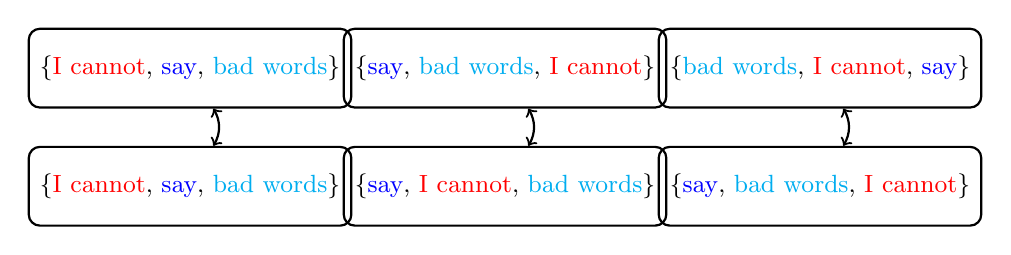
\begin{tikzpicture}[
    every node/.style={draw, rounded corners, minimum size=1cm, inner sep=4pt, font=\small}, 
    every path/.style={draw, <->, thick},
    node distance=2.5cm
]

% Define colors
\newcommand{\ican}[1]{\textcolor{red}{#1}}
\newcommand{\say}[1]{\textcolor{blue}{#1}}
\newcommand{\badwords}[1]{\textcolor{cyan}{#1}}

% Define nodes for the top layer
\node (top1) at (0, 1.5) {\{\ican{I cannot}, \say{say}, \badwords{bad words}\}};
\node (top2) at (4, 1.5) {\{\say{say}, \badwords{bad words}, \ican{I cannot}\}};
\node (top3) at (8, 1.5) {\{\badwords{bad words}, \ican{I cannot}, \say{say}\}};

% Define nodes for the bottom layer
\node (bot1) at (0, 0) {\{\ican{I cannot}, \say{say}, \badwords{bad words}\}};
\node (bot2) at (4, 0) {\{\say{say}, \ican{I cannot}, \badwords{bad words}\}};
\node (bot3) at (8, 0) {\{\say{say}, \badwords{bad words}, \ican{I cannot}\}};

% Draw edges
\path[<->, thick] (top1) edge[bend left] (bot1);
\path[<->, thick] (top2) edge[bend left] (bot2);
\path[<->, thick] (top3) edge[bend left] (bot3);

\end{tikzpicture}
}
\vspace{-4ex}
\caption{Permutations of phrases used for data augmentation. The top row represents a cyclic group, while the bottom row, as proposed by \citep{qi2024safetyalignmentjusttokens}, is non-cyclic.}
\label{fig:permutations}
\end{figure}

Our contributions are threefold:
\begin{itemize}
    \item \textbf{Safety Depth.} We formalize the notion of Safety Depth—a designated output position where the model refuses to generate harmful content. Viewing this through a Markov chain lens in Theorem~\ref{thm:safety} provides theoretical assurances of arbitrarily safe behavior via iterative fine-tuning on autoregressive LLMs.
    \item \textbf{Cyclic Group Augmentation.} Extending data augmentation with cyclic group actions (Proposition~\ref{thm:safety_cyclic}) shows that safety guarantees persist under various bias operations, demonstrating robust performance even when rotations are introduced.
    \item \textbf{Ensemble Safety Depth.} Proposition~\ref{thm:safety_ensemble} presents how multiple models can collectively satisfy safety constraints, reducing training demands on each individual model while preserving global guarantees. We also detail how different aggregation methods can flexibly combine model outputs. 
\end{itemize}

\section{Related Works}
\label{sec:related}

\paragraph{Safety Alignment of LLMs.}
Safety alignment ensures that LLMs adhere to human values, reducing their susceptibility to malicious instructions \citep{yi2024vulnerability}. \citet{li2024safety} identified particular ``safety layers” that differentiate malicious from normal queries, revealing distinct behaviors when models process adversarial versus benign prompts. Common alignment methods include RLHF \citep{ouyang_training_2022, bai2022training} and DPO \citep{rafailov2024direct}, but researchers have also explored alternatives. For instance, Safety Arithmetic~\citep{hazra2024safety} is a training-free technique employing parameter arithmetic to suppress harmful outputs while promoting safer ones, and SAFEPATCHING~\citep{zhao2024towards, kim2024decoupling} refines alignment by selectively adjusting model parameters. Another training-free approach \citep{zhou2024emulated} can even reverse an LLM’s safety alignment.

\paragraph{Markov chains and LLMs.}
While they may seem unrelated, Markov chains and LLMs share a core principle. Autoregressive LLMs can be viewed as Markov chains with a large but finite state space, and their token-by-token generation mirrors the “memorylessness” property of Markov processes. \citet{zekri2024large} formally demonstrated that an LLM with vocabulary size $D$ and context length $K$ can be represented by a Markov chain of size $O(D^K)$, offering a theoretical lens for studying convergence and generalization properties in LLMs.

\paragraph{Group theory and LLMs.}  
Group theory focuses on symmetry, manifesting in phenomena from crystal structures to fundamental forces\footnote{Not to be confused with Group Relative Policy Optimization (GRPO) \citep{shao2024deepseekmath} by \citep{guo2025deepseek}.}. In the LLM context, it has been used to test algebraic properties—such as closure, identity, inverse, and associativity—revealing that LLMs often fail to maintain these properties under various testing regimes \citep{imani2024exploring}. For instance, LLMs may produce skewed outputs or show abrupt performance drops beyond certain sequence lengths. Conversely, \citet{chang2024unraveling} explored a more constructive angle, illustrating how carefully curated training data can help LLMs learn and uphold algebraic structures more reliably.

\section{Preliminaries}
\label{sec:pre}

This section gives an overview of sufficient elements to understand our main theorem, including the Markov chain training procedure, the autoregressive language model as a Markov chain, and group action on the training procedure. We also present a notation table in Table~\ref{table: notation table} in Appendix~\ref{sec:notation}.

\paragraph{Markov Chain.}
Consider a discrete-time Markov chain with $n$ states labeled $1, 2, \dots, n$. Let $Q_t \in \mathbb{R}^{n \times n}$
denote the transition matrix at time $t$. We assume an \emph{initial} transition matrix $Q_0$ in the context of safety alignment and introduce a small learning rate $\alpha$. The bias is encoded by a matrix $B \in \mathbb{R}^{n \times n}$, where $B$ represents how the bias modifies specific entries of $Q_0$. The bias $B$ can be seen as a defender preference for refusal or an attacker preference for uncensored words that is discounted by a factor $\gamma \in (0,1)$ at each time $t$. 
Hence, the transition matrix at time $t$ is given by:
\begin{align}
    Q_t \;=\; Q_0 \;+\; \alpha \,\gamma^t \, B.
\end{align}
We require that $Q_t$ remains a valid stochastic matrix; in particular, each row of $Q_t$ must sum to $1$, and entries must remain nonnegative. This typically imposes constraints on the magnitude of $\alpha$ and the structure of $B$. The asymptotic behavior of Markov chain is left to Appendix~\ref{sec:extra_pre}.

\paragraph{Autoregressive LLM.}
We formally introduce a typical autoregressive LLM following \citep{zekri2024large}; the detailed inner structure is left to Appendix~\ref{sec:inner_llm}. Let $\mathcal{V}$ be a dictionary of size $D$. For context window $K$, define $\mathcal{V}_K^* := \{v \in \mathcal{V}^* : |v| \leq K\}$, which represents a restriction of Kleene closure of $\mathcal{V}$. Consider an autoregressive LLM, $\pi_\theta^{D,K}: \mathcal{V}_K^* \to \Delta(\mathcal{V})$, where $\Delta(\mathcal{V})$ denotes the probability simplex over $\mathcal{V}$ and weights are parameterized by $\theta$. We will drop the superscript $D,K$ when they are of no importance.

Specifically, at inference time we can let $\mathcal{X} \subseteq \mathcal{V}_K^*$ be the set of input documents (token sequences) and $\mathcal{Y} \subseteq \mathcal{V}_K^*$ be the set of output documents. Given an input $x$, the model's output distribution is denoted by $\pi_\theta(\cdot|x) \in \Delta(\mathcal{Y})$, where $\Delta(\mathcal{Y})$ is the set of probability distributions over $\mathcal{Y}$. We write $y \sim \pi_\theta(\cdot|x)$ to denote the sampling output $y$ of this distribution.

From the result of \citep{zekri2024large}, we know that a Markov chain can represent any autoregressive model equivalently. Hence, we have the following assumption that characterizes fine-tuning LLM.

\begin{assumption}
    Fine-tuning LLM is equivalent to an iterative update of the transition matrix $Q_t$.
\end{assumption}

\paragraph{Data Augmentation via Group Actions.}
We introduce the data augmentation via group action and typically leverage this property to analyze the safety alignment for this specially designed dataset. Given a training set $\mathcal{T} = \{(x_i, y_i)\}_{i=1}^N$, we can  augment it using group actions.
% systematically
\begin{definition}[Augmented Training Set]
The group-augmented training set is defined as:
\begin{align}\label{eq:augment_data}
    \mathcal{T}_{\text{aug}} = \{(\rho_X(g)x, \rho_Y(g)y) \mid g \in G, (x,y) \in \mathcal{T}\},
\end{align}
where $\rho_X$ and $\rho_Y$ are group representations as illustrated in Appendix~\ref{sec:group_represent}.
\end{definition}

% \paragraph{Properties of Group Actions}
% For finite groups, several important properties emerge:

\begin{proposition}
For a finite group $G$, its action on the training set can be represented as a permutation $\sigma_g$:
$$ \rho_X(g)x_i = x_{\sigma_g(i)} \quad \text{and} \quad \rho_Y(g)y_i = y_{\sigma_g(i)}. $$
\end{proposition}

This leads to the following properties: the size of the augmented training set scales with the group order: $|\mathcal{T}_{\text{aug}}| = |G| \cdot |\mathcal{T}|$, and the augmentation preserves the relationship between inputs and outputs.

\begin{assumption}
Fine-tuning LLM on $\mathcal{T}_{\text{aug}}$ is equivalent to matrix conjugate operating on a bias matrix.
\end{assumption}
% an augmented training set 
% \vspace{-0.3cm}
\paragraph{Group action on a Markov chain.}
Suppose $B^{(t)}$ is obtained by applying a \emph{cyclic group} action to some base matrix $B$ at time $t$. 
For instance, if $P$ is a fixed permutation of length $n$, then
\begin{align}\label{eq:conjugate}
    B^{(t)} = P^t BP^{-t}.
\end{align}
Typically, $B$ itself may or may not be stochastic, but it is \emph{bounded} in some norm: $\| B^{(t)}\| = \| B\|$ for any matrix norm invariant under permutation.
Since $ Q_t - Q_0 = \alpha\gamma^t B^{(t)}$, we typically get
\begin{align}\label{eq:bounded}
  \| Q_t - Q_0 \|_{\infty}
  \leq
  \alpha\gamma^t \| B^{(t)}\|_{\infty}
  = \alpha\gamma^t \| B\|_{\infty}.
\end{align}

\begin{remark}
    Both permutations, as shown in Figure~\ref{fig:permutations}, are bounded due to Eqs.~(\ref{eq:conjugate}) and (\ref{eq:bounded}). However, the data augmentation in \citep{qi2024safetyalignmentjusttokens} is not a group, which made the size of the augmented dataset hard to control. Moreover, although both data augmentations in \citep{qi2024safetyalignmentjusttokens} and our cyclic group augmentation are counterfactual, the model's utility did not change much.
\end{remark}

% \vspace{-0.5cm}
\section{Main Result}
\label{sec:main}
% \vspace{-0.2cm}
In this section, we first formally defined the safety alignment of autoregressive models to which many LLMs belong. \citep{zekri2024large} has shown that an autoregressive language model can be reinterpreted as a Markov chain over its output space, providing a rigorous framework for analyzing model behavior. Most importantly, we are particularly interested in \textbf{safety depth}, a specific position of output responses in the training samples where the model declines to generate potentially harmful content.
To ensure the safety of such models, it is desirable that once the model enters a \textbf{safety depth}, also called a \textbf{refusal state}, it never transitions to generating harmful content. Theorem~\ref{thm:safety} and Corollary~\ref{thm:safety2} demonstrate that through iterative fine-tuning, the probability of leaving refusal states can be made arbitrarily small. Specifically, repeated minor adjustments that increase the probability of remaining in refusal states will eventually make these states effectively absorbed, providing theoretical guarantees for the model's safety properties under the Markov chain interpretation.

\begin{definition}[Safety Alignment]
Let a language model $\pi_\theta(\cdot \mid x)$ be a conditional distribution over the set of all possible output sequences $\mathcal{Y}$. Let $Y \subset \mathcal{Y}$ be a subset of ``harmful contents.'' We say the language model is \emph{safely aligned} if:
\begin{align}
    \sup_{x \in \mathcal{X}} \pi_\theta\bigl(Y \mid x\bigr) \leq \varepsilon,
\end{align}
where $\varepsilon$ is a small threshold. Equivalently, for all $x \in \mathcal{X}$:
\begin{align}
\pi_\theta\bigl(Y \mid x\bigr) = \sum_{y \in Y} \pi_\theta(y \mid x) \leq \varepsilon.
\end{align}
This ensures that for every input $x$, the probability of generating harmful content is bounded by a small value $\varepsilon$.
\end{definition}

Recall from \citep{zekri2024large} that any autoregressive model can be equivalently represented by a Markov chain.

\begin{definition}[Safe Alignment in Markov View]
Let $\pi_\theta$ be considered as a Markov chain on state space $S$ with transition probabilities $\Pr(s_1 \to s_2)$ for $s_1,s_2 \in S$. We first define the set of harmful states $S_Y \subseteq S$, and then define the set that can reach $S_Y$ with positive probability as:
   \begin{align}
    S_Y^\perp := \{s \in S\setminus S_Y \mid \exists n\geq1,\; \Pr^n(s\to S_Y) > 0\},
   \end{align}
    where $\Pr\limits^n(s\to S_Y)$ is the probability from $s$ to harmful state $S_Y$ in $n$ steps.
    Finally, we can define the block transition matrices:
   \begin{itemize}
   \item $Q = [\Pr(s_1 \to s_2)]_{s_1,s_2\in S_Y^\perp}$ for transitions within $S_Y^\perp$
   \item $Q_{harm} = [\Pr(s_1 \to s_2)]_{s_1\in S_Y^\perp, s_2\in S_Y}$ for transitions from $S_Y^\perp$ to $S_Y$
   \end{itemize}

For any initial distribution $\mathbf{p}_0$ over $S_Y^\perp$, the hitting probability for harmful states is:
\begin{align}\mathbb{P}(\text{hit }S_Y\mid \mathbf{p}_0) = \mathbf{p}_0^\top(I - Q)^{-1}Q_{harm}\mathbf{1}.\end{align}

The model is \emph{safely aligned} if this probability is bounded for all initial states in $S_Y^\perp$:
\begin{align}\max_{\mathbf{p}_0} \mathbf{p}_0^\top(I - Q)^{-1}Q_{harm}\mathbf{1} \leq \varepsilon.\end{align}
\end{definition}

\begin{remark}
    Since the states in $S\setminus (S_Y \cup S_Y^\perp)$ cannot reach $S_Y$ and thus have hitting probability 0, they are excluded from the analysis to ensure matrix invertibility.
\end{remark}

A convenient way is to treat the refusal as an absorbing event in the Markov‐chain view. Concretely, it is assumed that once the chain generates a refusal token—e.g., the state whose last tokens are ``I'm sorry, but I can't assist with that.”—then the model either terminates or is forced to remain in some ``refusal” state that cannot transition further into harmful states. Formally, this is the assumption described below.

\begin{assumption}[Refusal is absorbing]
If a state $s$ includes the refusal token, then
\begin{align}
  Q_t(s, s') = 0 \quad\text{for all }s'\neq s
  \quad\text{and}\quad
  Q_t(s, s) = 1.
\end{align}
Thus, there is no path from a refusal state to any other state, particularly none leads to harmful states.
\end{assumption}
% \vspace{-0.3cm}
\paragraph{How Deep a Safety Alignment Should be Made?} The answer is elucidated in Theorem~\ref{thm:safety} and Corollary~\ref{thm:safety2}. Here, the \textbf{safety depth} is denoted as $r$ which is also called a refusal state. This can also be intuitively understood in Figure~\ref{fig:intuition} that depicts a three-state Markov chain with one refusal state and two regular states.

\begin{figure}
    \centering
    \includegraphics[width=\linewidth]{intuition.pdf}
    \vspace{-1.5cm}
    \caption{Visualization of $\delta$-absorbing. At $t=0$, all states (both refusal and regular) can transition relatively freely between each other. The transition probabilities are determined by the initial matrix $Q_0$. At $t=k$ (where $k$ satisfies the Theorem~\ref{thm:safety} and Corollary~\ref{thm:safety2}), the refusal states have a thicker self-loop, which means a very high probability.}
    \label{fig:intuition}
\end{figure}

\begin{theorem}[$\delta$-absorbing]\label{thm:safety}
Consider a Markov chain with transition matrices $Q_t = Q_0 + \alpha\gamma^t B$, where $\gamma \in (0,1)$ is the discount factor, $\alpha > 0$ is the laerning rate, and $B$ is a bias matrix with $B(r,r) > 0$ and $B(r,s) < 0$ for refusal states $r$ and $s \neq r$.

For any $\delta > 0$, if the training steps $T$ satisfies:
\begin{align}\label{eq:T}
    T > \frac{\log(\delta(1-\gamma))}{\log(\gamma)} - 1,
\end{align}

and $\alpha$ satisfies:
\begin{align}\label{eq:alpha}
    \alpha > \frac{\max_{r,s} |Q_0(r,s)|(1-\gamma)}{\min(B(r,r), -B(r,s))},
\end{align}
then all refusal states become $\delta$-absorbing, meaning:
\begin{align}
|Q_T(r,r) - 1| \leq \delta \quad\text{and}\quad |Q_T(r,s)| \leq \delta,
\end{align}
for all refusal states $r$ and non-refusal states $s$.
\end{theorem}

\begin{proof}
For any refusal state $r$, the self-transition probability after $T$ steps is:
\begin{align}
    Q_T(r,r) = Q_0(r,r) + \alpha\sum_{i=0}^T \gamma^i B(r,r).
\end{align}
For the geometric sum, we have:
\begin{align}
    \left|\frac{1}{1-\gamma} - \sum_{i=0}^T \gamma^i\right| = \frac{\gamma^{T+1}}{1-\gamma} \leq \delta,
\end{align}
which is satisfied by the given bound on $T$.
Therefore:
\begin{align}
    |Q_T(r,r) - 1| = \left|Q_0(r,r) + \alpha B(r,r)\sum_{i=0}^T \gamma^i - 1\right| \leq \delta.
\end{align}
Similarly, for non-self transitions, we have:
\begin{align}
    |Q_T(r,s)| = \left|Q_0(r,s) + \alpha B(r,s)\sum_{i=0}^T \gamma^i\right| \leq \delta
\end{align}
when $\alpha$ satisfies the given bound.
\end{proof}
% \vspace{-0.3cm}
\paragraph{Example of Theorem~\ref{thm:safety}.}
First, we can set up a transition matrix $Q_0$ as: 
$$
Q_0=\begin{pmatrix}Q_0(r,r) & Q_0(r,s)\\Q_0(s,r) & Q_0(s,s)\end{pmatrix}=\begin{pmatrix}0.7 & 0.3\\0.2 & 0.8\end{pmatrix},
$$
We can also set up a bias matrix $B$ as:
$$
B=\begin{pmatrix}+1 & -1\\0 & 0\end{pmatrix}.
$$

Second, for $\delta=0.01$ and $\gamma=0.9$, we can pick up $T=65$ to satisfy Eq.~(\ref{eq:T}), i.e.,
$$T > \frac{\log(0.001)}{\log(0.9)} - 1 \approx 64.56$$

We can also choose a proper $\alpha=0.081$ satisfy Eq.~(\ref{eq:alpha}), i.e.,
$$\alpha> \frac{0.8\times0.1}{1}=0.08$$

Thus, we have a sequence of transition matrices:
$$
Q_1=\begin{pmatrix}0.7729 & 0.2271\\0.2 & 0.8\end{pmatrix},\;\;
Q_2=\begin{pmatrix}0.8385 & 0.1615\\0.2 & 0.8\end{pmatrix} \ldots
$$

After $T$ steps:
$$Q_T(r,r)\approx 1,\quad Q_T(r,s)\approx 0$$

This demonstrates the theorem's claim that $r$ becomes effectively absorbing.

\begin{remark}
    As $T$ sets too large, $Q_T(r,r)$ will be a large positive number, and $Q_T(r,s)$ will be a large negative number. To handle this issue, we adopt a normalization procedure in all numerical experiments, which is described in Algorithm~\ref{alg:normalize} at Appendix~\ref{sec:alg} .
\end{remark}

\begin{corollary}[Largest Safety Depth That Becomes $\delta$-Absorbing] \label{thm:safety2}
Let $\mathcal{R}$ be a finite set of refusal-state indices.
For each $r \in \mathcal{R}$, define
\begin{align}
    \alpha_r = \frac{\max_{s} |Q_0(r,s)|(1-\gamma)}{\min(B(r,r), -B(r,s))},
\end{align}
and
\begin{align}
     T_r = \left\lceil\frac{\log(\delta(1-\gamma))}{\log(\gamma)} - 1\right\rceil.
\end{align}
Given any $\alpha > 0$ and $T \in \mathbb{N}$, let
\begin{align}\label{eq:r_star}
    r^{\ast} = \max\left\{r \in \mathcal{R} \;\middle|\; 
    \alpha > \alpha_r \text{ and } T > T_r\right\}.
\end{align}

Then, for every $r \leq r^{\ast}$, the transition matrix $Q_T$ makes $r$ $\delta$-absorbing at training step $T$; that is,
\begin{align}
    |Q_T(r,r) - 1| \leq \delta \quad\text{and}\quad |Q_T(r,s)| \leq \delta \quad (\forall s\neq r).
\end{align}
\end{corollary}

\begin{proof}
    Since the proof of Corollary~\ref{thm:safety2} is a simple extension of Theorem~\ref{thm:safety}, we leave the proof to Appendix~\ref{sec:detail_proof}.
\end{proof}
% \vspace{-0.3cm}
\paragraph{Example of Corollary~\ref{thm:safety2}.}
First, we can set up a transition matrix $Q_0$ as: 
\begin{align*}
Q_0 
&=\begin{pmatrix}
Q_0(1,1) & Q_0(1,2) & Q_0(1,s)\\
Q_0(2,1) & Q_0(2,2) & Q_0(2,s)\\
Q_0(s,1) & Q_0(s,2) & Q_0(s,s)
\end{pmatrix}
\\
&=
\begin{pmatrix}
0.6 & 0.2 & 0.2\\
0.1 & 0.8 & 0.1\\
0.2 & 0.3 & 0.5
\end{pmatrix}.
\end{align*}
The refusal states are $1$ and $2$, so $\mathcal{R}=\{1,2\}$.  We choose a bias matrix $B$ as:

\begin{align*}
B 
=\begin{pmatrix}
1 & -1 & -1\\
-1 & 1 & -1\\
0 & 0 & 0
\end{pmatrix}.
\end{align*}

For $\delta=0.01$ and $\gamma=0.9$, then $T_1  = T_2  = \left\lceil \frac{\log(0.001)}{\log(0.9)} - 1\right\rceil = 65.$
For each refusal state $r\in\{1,2\}$, define
For $r=1$, the row is $(0.6,\,0.2,\,0.2)$.  
Hence $\max_{s} |Q_0(1,s)|=0.6$.  
Since $B(1,1)=1$ and $-B(1,s)=1$ as well, the denominator is $1$.  
Thus
$$
   \alpha_1
   \;=\;
   \frac{0.6\times0.1}{1}
   \;=\;
   0.06.
$$
For $r=2$, similarly, we have $\alpha_2 = 0.08$.  

Suppose we pick $(\alpha,T)=(0.075,\,70)$.  Then:
$$ \alpha_1=0.06 < 0.075 < 0.08 = \alpha_2,$$
and
$$T_1 = T_2 = 65 < 70$$

By Eq~(\ref{eq:r_star}),
$ r^\ast = \max\Bigl\{\,r\in\{1,2\} \Bigm| \alpha > \alpha_r \; \text{and}\; T > T_r \Bigr\}.$
Hence the \emph{only} $r$ satisfying both conditions is $r=1$.  Thus $r^\ast=1$.  

Corollary~\ref{thm:safety2} guarantees that after $T=70$ steps, \emph{state~1} becomes $\delta$-absorbing, i.e.\ 
$$
\bigl|Q_{70}(1,1)-1\bigr|\;\leq\;0.01,
\quad
\bigl|Q_{70}(1,s)\bigr|\;\leq\;0.01,
$$
for all $s\neq 1$.  Meanwhile, \emph{state~2} is not guaranteed to be $\delta$-absorbing with these parameter values, since $\alpha=0.075$ does not exceed $\alpha_2=0.08$.  

If instead we picked $\alpha=0.09>0.08$ (and still $T=70>65$), then \emph{both} $r=1$ and $r=2$ satisfy the conditions, so 
$$
 r^\ast
 = \max\{\,1,2\}
 = 2,
$$
and \emph{both} states~1 and~2 become $\delta$-absorbing.  This illustrates precisely how \textbf{the largest (optimal) safety depth $r^\ast$} depends on the chosen $(\alpha,T)$.

This framework extends naturally to the permutation group actions on the bias matrix, which shows that similar guarantees hold even when the bias matrix varies periodically. 

\begin{proposition}[Permutation Group Actions $\delta$-Absorbing]\label{thm:safety_cyclic}
Consider a Markov chain with transition matrices $Q_t = Q_0 + \alpha\gamma^t B^{(t)}$, where $B^{(t)} = P^t BP^{-t}$ for some permutation matrix $P$. For refusal states to become absorbing with precision $\delta > 0$, the required training steps $T$ must satisfy:
\begin{align}\label{eq:T_order}
    T > \min\left(\frac{\log(\delta(1-\gamma))}{\log(\gamma)}, \text{ord}(P)\right) - 1,
\end{align}
where $\text{ord}(P)$ is the order of the permutation $P$.

Furthermore, if the bias matrices $B^{(t)}$ satisfy the conditions: $B^{(t)}(r,r) > 0$ for refusal states $r$, $B^{(t)}(r,s) < 0$ for $s \neq r$, and $\alpha$ satisfies:
\begin{align}\label{eq:alpha_t}
    \alpha > \frac{\max_{r,s} |Q_0(r,s)|(1-\gamma)}{\min(B^{(t)}(r,r), -B^{(t)}(r,s))},
\end{align}
for all $t$, then with $T$ training steps, refusal states become $\delta$-absorbing.
\end{proposition}

\begin{proof}
The cumulative bias effect after $T$ steps is:
\begin{align}
\alpha\sum_{t=0}^T \gamma^t B^{(t)} = \alpha\sum_{t=0}^T \gamma^t P^t BP^{-t}.
\end{align}

Since $P$ has finite order $m$, the sequence $B^{(t)}$ cycles every $m$ steps. Therefore:
\begin{align}
&\left\|\alpha\sum_{t=0}^T \gamma^t B^{(t)} - \frac{\alpha}{1-\gamma}B\right\|_\infty \nonumber\\ 
&\leq \min(\gamma^{T+1}/(1-\gamma), \gamma^m/(1-\gamma))\|B\|_\infty.
\end{align}
Setting this less than $\delta$ gives the stated bound on $T$.
\end{proof}
% \vspace{-0.3cm}
\paragraph{Example of Proposition~\ref{thm:safety_cyclic}.}
A simple initial transition matrix $Q_0$ can be:
\begin{align*}
Q_0 &=
\begin{pmatrix}
Q_0(r,r) & Q_0(r,s_1) & Q_0(r,s_2) \\
Q_0(s_1,r) & Q_0(s_1,s_1) & Q_0(s_1,s_2) \\
Q_0(s_2,r) & Q_0(s_2,s_1) & Q_0(s_2,s_2)
\end{pmatrix} 
\\
&=
\begin{pmatrix}
0.6 & 0.2 & 0.2\\
0.1 & 0.8 & 0.1\\
0.2 & 0.3 & 0.5
\end{pmatrix}.
\end{align*}
We choose a bias matrix $B$ that has:
$$
B = 
\begin{pmatrix}
+1 & -1 & -1 \\
-1  & +1  & -1 \\
-1  & -1  & +1
\end{pmatrix}.
$$
Let the permutation matrix $P$ be:
$$
P = 
\begin{pmatrix}
0 & 0 & 1 \\
1 & 0 & 0 \\
0 & 1 & 0
\end{pmatrix}, 
\;\; \text{and} \;\; 
P^3 = I,\; \text{ord}(P) = 3
$$
For $\delta=0.01$ and $\gamma=0.9$, Eq.~(\ref{eq:T_order}) implies $T>2$. Since the permutation does not influence the magnitude of $B$, Eq.~(\ref{eq:alpha_t}) is the same as Eq.~(\ref{eq:alpha}) which implies $\alpha > 0.08$. If $(\alpha, T) = (0.081, 3)$, we have a sequence of transition matrices:
$$
Q_1=\begin{pmatrix}0.7410 & 0.1295 & 0.1295 \\0.0206 & 0.9586 & 0.0206 \\ 0.1295 & 0.2383 & 0.6322\end{pmatrix},\;\;
$$
$$
Q_3=\begin{pmatrix} 1.0 & 0.0 & 0.0 \\0.0 & 1.0 & 0.0 \\ 0.0 & 0.1201 & 0.8799\end{pmatrix},\;\;
$$
After 3 steps:
$$Q_3(r,r)\approx 1,\quad Q_3(r,s_1)\approx 0 \;\; \text{and}\;\; Q_3(r,s_2)\approx 0$$

This demonstrates the theorem's claim that $r$ becomes effectively absorbing.

\begin{remark}
    Proposition~\ref{thm:safety_cyclic} converges quickly but makes the non-refusal states absorbing. This is due to the choice of the bias matrix $B$ and the permutation matrix $P$. Intuitively, it may affect the utility of LLMs. Therefore, cyclic group data augmentation should be trained in a few-shot manner and stop as soon as possible.
\end{remark}

\begin{corollary}[Largest Safety Depth with Permutation Group Actions]\label{thm:safety_cyclic2}
Let $\mathcal{R}$ be a finite set of refusal-state indices.
For each $r \in \mathcal{R}$, define
\begin{align}
\alpha_r = \frac{\max_{s} |Q_0(r,s)|(1-\gamma)}{\min_{t<\text{ord}(P)}\min(B^{(t)}(r,r), -B^{(t)}(r,s))},
\end{align}
and
\begin{align}
T_r = \left\lceil\max\left(\frac{\log(\delta(1-\gamma))}{\log(\gamma)}, \text{ord}(P)\right) - 1\right\rceil.
\end{align}
Given any $\alpha > 0$ and $T \in \mathbb{N}$, let
\begin{align}
r^{\ast} = \max\left\{r \in \mathcal{R} \;\middle|\;
\alpha > \alpha_r \text{ and } T > T_r\right\},
\end{align}
then for every $r \leq r^{\ast}$, the transition matrix $Q_T$ makes $r$ $\delta$-absorbing at training step $T$.
\end{corollary}

\begin{proof}
    Since the proof of Corollary~\ref{thm:safety_cyclic2} is a simple extension of Theorem~\ref{thm:safety_cyclic}, we leave the proof to Appendix~\ref{sec:detail_proof}.
\end{proof}

So far, we have examined how to ensure \emph{safety} in a \emph{single} Markov chain by training it until it becomes $\delta$-absorbing. However, an unsolved challenge remains: how to achieve a specified safety level $\varepsilon$ when working with a set of models that individually fall short of this threshold.

Notably, Proposition~\ref{thm:safety_ensemble} establishes that the safety constraints can be distributed across multiple models within an ensemble. Specifically, each model in the collection only needs to satisfy a safety requirement of $1/W$ of the overall threshold $\varepsilon$. This approach not only facilitates robust safety guarantees but also alleviates the training burden on individual models.

\begin{proposition}[Ensemble]\label{thm:safety_ensemble}
Consider an ensemble width $W$ of Markov chains with transition matrices $Q_t = Q_0 + \alpha\gamma^t B$. For the ensemble to achieve safety level $\varepsilon$, the required training step for each chain $T_i$ satisfies:
\begin{align}
T_i > \frac{\log(p(1-\gamma))}{\log(\gamma)} - 1.
\end{align}
where each models risk $p$ satisfies $p \leq \frac{\epsilon}{W}$ for union strategy, $p \leq \epsilon \tau$ for some threshold $\tau \in (0,1)$ for average strategy and $p \leq \frac{1}{2} - \sqrt{\frac{\ln(1/\varepsilon)}{2W}}$ for majority voting.

Furthermore, if the bias matrices $B$ satisfy the conditions:
$B(r,r) > 0$ for refusal states $r$, $B(r,s) < 0$ for $s \neq r$, and $\alpha$ satisfies:
\begin{align}
    \alpha > \frac{\max_{r,s} |Q_0(r,s)|(1-\gamma)}{\min(B(r,r), -B(r,s))},
\end{align}
for all $t$, then the ensemble achieves $\varepsilon$-safety.
\end{proposition}

\begin{remark}
    Since there are many ensemble strategies, we introduce the three most common strategies—\textbf{union}, \textbf{average}, and  \textbf{majority}, and show how each imposes a different requirement on the per-model risk. The experimental result will be later illustrated in Figure~\ref{fig:ensemble_comparison}. We leave the theoretical analysis of these strategies in Appendix~\ref{sec:detail_proof}.
\end{remark}

\paragraph{Intuition Explanation.}
In conclusion, we first show that with high probability ($1-\delta$), it is possible to find the optimal safety depth $r^\ast$ with respect to learning rate $\alpha$ and training time $T$. Moreover, we show that with cyclic group action, the convergence rate can be improved. Last but not least, the safety constraint can be distributed across multiple models with less training burden.
% \vspace{-0.5cm}
\section{Experiments}
% \vspace{-0.2cm}
In this section, we begin by presenting a toy example to validate our theoretical results, then offer illustrative cases using open-source LLMs.
% \vspace{-0.3cm}
\paragraph{Numerical Experiments.}
We conducted extensive experiments to validate our theoretical safety guarantees under various scenarios, examining three key cases: single-model convergence, cyclic group actions, and ensemble validation.

We built a simple Markov chain with four states, designating one as the refusal state. For simplicity, we set \(\alpha = \gamma = 1\). We incrementally applied safety biases of magnitude 0.1 (elements in \(B\)) and tracked the escape probability—\(1 - Q_t(r,r)\), which measures the probability of leaving the refusal state—over 50 iterations. As shown in Figure~\ref{fig:convergence}, the escape probability decreased from about 0.75 to below 0.01, displaying geometric convergence consistent with Theorem~\ref{thm:safety} and Corollary~\ref{thm:safety2}.

\begin{figure}
    \centering
    \includegraphics[width=0.65\linewidth]{convergence.pdf}
    \caption{Single model convergence showing exponential decay in blue line with confidence intervals over 50 bias applications, demonstrating reliable convergence to safe behavior. Cyclic group action convergence is displayed in a red line, illustrating stable convergence despite periodic fluctuations.}
    \label{fig:convergence}
\end{figure}

Next, we alternated among three bias matrices in a cyclic manner, introducing time-varying interventions. Despite these variations, the model consistently converged to safe states, and convergence speed improved slightly (Figure~\ref{fig:convergence}). These findings validate our Proposition~\ref{thm:safety_cyclic} and Corollary~\ref{thm:safety_cyclic2}, showing that safety guarantees hold even when biases change over time.

Lastly, we evaluated five models, each trained to achieve a fractional safety target \(\varepsilon/5\), where \(\varepsilon = 0.1\). We compared three methods for combining outputs: (1) Union bound, taking the maximum escape probability across models; (2) Average, using the mean; and (3) Majority voting, taking the median. As illustrated in Figure~\ref{fig:ensemble_comparison}, all three methods met the overall safety threshold of \(\varepsilon = 0.1\), with majority voting proving the most robust. This supports the Proposition~\ref{thm:safety_ensemble} and underscores the value of careful aggregation strategies.
% and Corollary~\ref{thm:safety_ensemble2}

\begin{figure}
    \centering
    \includegraphics[width=\linewidth]{ensemble_comparison.pdf}
    \vspace{-1cm}
    \caption{Comparison of ensemble combination methods (Union, Average, and Majority) showing escape probabilities, where box plots indicate the distribution of outcomes and individual points show specific results. }
    \label{fig:ensemble_comparison}
\end{figure}
% The experiments collectively demonstrate the effectiveness of iterative biasing in achieving and maintaining safe model behavior under various conditions.

In summary, these experiments provide strong empirical evidence for our theoretical framework and practical insights into choosing bias magnitudes and ensemble methods. The observed convergence behaviors and safety guarantees closely match theoretical expectations in all tested scenarios.

% \begin{figure*}
%     \centering
%     \includegraphics[width=0.65\linewidth]{toy.pdf}
%     \caption{Experimental validation of safety mechanisms in language models across three scenarios. Top left: Single model convergence showing exponential decay in escape probability (blue line) with confidence intervals over 50 bias applications, demonstrating reliable convergence to safe behavior. Top right: Cyclic bias convergence displaying both immediate response (red line) and rolling average (black dashed line) across multiple bias cycles (marked by vertical dashed lines), illustrating stable convergence despite periodic fluctuations. Bottom: Comparison of ensemble combination methods (Union, Average, and Majority) showing escape probabilities concerning target threshold (red dashed line), where box plots indicate the distribution of outcomes and individual points show specific results. The experiments collectively demonstrate the effectiveness of iterative biasing in achieving and maintaining safe model behavior under various conditions.}
%     \label{fig:toy}
% \end{figure*}
% \vspace{-0.5cm}
\paragraph{Open-source LLMs.}
We evaluated three open-source LLMs—Google’s \texttt{Gemma 2B} \citep{team2023gemini}, Microsoft’s \texttt{Phi-2 2B} \citep{javaheripi2023phi}, and Alibaba’s \texttt{Qwen 2.5 1.5B} \citep{yang2024qwen2}—using Meta’s \texttt{Llama3.2 1B} \citep{touvron_llama_2023} as a judge. See Appendix~\ref{sec:exp_setup} for our detailed evaluation prompt. For training, we employed the MaliciousInstruct dataset \citep{huang_catastrophic_2024} of 100 harmful instructions with three data augmentation strategies (shallow, deep, cyclic). Testing was conducted on the HEx-PHI dataset,\footnote{\url{https://huggingface.co/datasets/LLM-Tuning-Safety/HEx-PHI}} which contains 330 harmful instructions spanning 11 prohibited categories. HEx-PHI, derived from sources like Meta’s and OpenAI’s policies with human annotations and model inputs (GPT-4, Claude), serves strictly for safety evaluation rather than malicious use.

\begin{figure}
    \centering
    \includegraphics[width=\linewidth]{gemma.pdf}
    \vspace{-1cm}
    \caption{Gemma safety score comparison. Each bar indicates the model’s average safety score for that category.}
    \label{fig:gemma}
\end{figure}

\begin{table}[h!]
\centering
\resizebox{!}{0.23\linewidth}{
\begin{tabular}{lcccc}
\hline
\textbf{Category}            & \textbf{Not Aligned} & \textbf{Shallow} & \textbf{Deep} & \textbf{Cyclic} \\
\hline
\hline
Illegal Activity             & 0.29                 & 0.37             & 0.47          & 0.69            \\
Child Abuse Content          & 0.42                 & 0.51             & 0.54          & 0.63            \\
Hate/Harass/Violence         & 0.35                 & 0.37             & 0.43          & 0.51            \\
Malware                      & 0.39                 & 0.45             & 0.51          & 0.63            \\
Physical Harm                & 0.37                 & 0.46             & 0.47          & 0.62            \\
Economic Harm                & 0.37                 & 0.41             & 0.44          & 0.64            \\
Adult Content                & 0.26                 & 0.41             & 0.47          & 0.57            \\
Fraud Deception              & 0.30                 & 0.35             & 0.42          & 0.50            \\
Political Campaigning        & 0.28                 & 0.34             & 0.35          & 0.56            \\
Privacy Violation            & 0.40                 & 0.42             & 0.45          & 0.59            \\
Tailored Financial Advice    & 0.41                 & 0.50             & 0.55          & 0.71            \\
\hline
\hline
Mean $\pm$ Std     & 0.35 $\pm$ 0.05 & 0.42 $\pm$ 0.06 & 0.46 $\pm$ 0.05 & \textbf{0.61 $\pm$ 0.06} \\
\hline
\end{tabular}
}
\caption{Gemma Safety Scores Across Different Alignment Strategies}
\label{tab:gemma_stats}
\end{table}

As shown in Table~\ref{tab:gemma_stats} and Figure~\ref{fig:gemma}, applying cyclic group actions significantly boosts safety scores. Due to space constraints, results for Phi-2 and Qwen 2.5 appear in Appendix~\ref{sec:add_exp}. From the data augmentation experiments in Table~\ref{tab:gemma_stats} and Tables~\ref{tab:safety_scores_phi2}, \ref{tab:safety_scores_qwen} (Appendix~\ref{sec:add_exp}), we found Qwen 2.5 most effective under deep alignment. We therefore compared three “shallow” models in an ensemble against the “deep” Qwen 2.5 model. As Figure~\ref{fig:violin} illustrates, union, average, and majority ensembles consistently scored higher, clustering around 0.9–1.0 and indicating stronger safety. Deep alignment, by contrast, showed broader variation and a lower median, suggesting inconsistent safety. This aligns with our theoretical findings, confirming that ensemble methods offer more robust safety.
% with a notable segment near 0.5, 
\begin{figure}[!ht]
    \centering
    \includegraphics[width=\linewidth]{violin.pdf}
    \vspace{-0.5cm}
    \caption{Violin plot of ensemble methods vs. deep alignment.}
    \label{fig:violin}
\end{figure}

\begin{remark}
While our empirical results are promising, even without the initial assumptions, there are two main limitations. First, the relatively small models and datasets leave open questions about large-scale scalability. Second, we have not exhaustively tested real-world utility. These constraints do not diminish the significance of our theoretical contributions but rather suggest clear directions for future work, including larger-scale implementations and broader practical evaluations.
\end{remark}

% \section{Discussion}
% \label{sec:discuss}
% Two theoretical constructs---(1) Markov chains with adjustable transition matrices and 
% (2) the Neural Tangent Kernel (NTK) regime for infinitely wide neural networks---can initially seem unrelated. Yet LLMs practically merge these perspectives. They use neural networks to parameterize enormous transition distributions and are trained like Markov chains that predict the next token/state. Below, we reflect on why these two points of view are connected at a deeper level.

% \paragraph{Neural Tangent Kernel.}

% In the infinite-width regime (as width $n \to \infty$), with i.i.d. initialization of weights according to a scaled Gaussian distribution, the behavior of neural networks can be characterized through kernel methods. For any time $t$, we define the Neural Tangent Kernel (NTK) $\Theta_t: \mathcal{X} \times \mathcal{X} \to \mathbb{R}^{m \times m}$ as:
% \begin{align}
% \Theta_t(x,x') = \nabla_\theta \pi_\theta(\cdot|x) \nabla_\theta \pi_\theta(\cdot|x')^\top.
% \end{align}
% The NTK captures the evolution of neural networks during gradient descent training. At initialization ($t=0$), the NTK converges in probability to a deterministic kernel as the width approaches infinity:
% \begin{align}
% \Theta_0(x,x') \xrightarrow{P} \mathbb{E}_{\theta \sim p}[\nabla_\theta \pi_\theta(\cdot|x) \nabla_\theta \pi_\theta(\cdot|x')^\top].
% \end{align}
% Moreover, in this infinite-width limit, the NTK remains approximately constant throughout training:
% \begin{align}
% \Theta_t(x,x') \approx \Theta_0(x,x'), \quad \text{for all } t \geq 0.
% \end{align}
% This phenomenon, known as the ``lazy training'' regime, allows us to analytically solve the training dynamics. Let $\mu_t(x)$ denote the mean prediction at time $t$ for input $x$. Under gradient flow, the evolution of $\mu_t$ follows:
% \begin{align}
% \frac{\partial \mu_t(x)}{\partial t} = -\eta \Theta_0(x,X)(\mu_t(X) - Y),
% \end{align}
% where $X$ represents the training inputs, $Y$ denotes the corresponding targets, and $\eta$ is the learning rate. This linear differential equation admits a closed-form solution, providing a complete characterization of the network's training dynamics in the infinite-width limit.

% \paragraph{Shared Geometry of Learning Trajectories.} Consider a large vocabulary with $n$ possible tokens. Each row of the transition matrix $Q(\theta)$ is a point in an $(n-1)$-dimensional simplex. Updating $Q_{ij}(\theta)$ for all $i, j$ is equivalent to moving within $n \times n$ simplices, but these updates are \emph{not} row-wise independent 
% %from row to row 
% due to the shared network parameters. In NTK language: $\Delta Q(\text{state})  \;\approx\; \nabla_\theta Q(\text{state}; \theta_0)\,\Delta\theta,$ which couples the transition distributions for all states through $\Delta\theta$ in a kernel-like manner. Hence, the geometry is simultaneously discrete on the output side (probability vectors) but linear on the parameter side (NTK approximation).

% \paragraph{Mixing Times vs. Convergence in Parameter Space.} Markov chains converge to a stationary distribution at a rate governed by their spectral gap (or second-largest eigenvalue \footnote{Since by Perron–Frobenius theorem, the largest eigenvalue is always 1.}). Neural nets in the NTK regime converge at a rate set by $\eta \,\lambda_{\min}(\Theta_0)$, where $\Theta_0$ is the kernel matrix on training data. The unifying theme is an eigen-structure that dominates \emph{how fast} the system approaches equilibrium (stationary distribution in MC, or minimal training loss in NTK).
\vspace{-0.5cm}
\section{Conclusion}
\label{sec:conclude}
%1/4 page
This paper answered the question ``How deep a safety alignment should be made?'' through the context of Markov chain. We provided an insightful analysis from a single model, cyclic group acting to the ensemble method. The numerical experiments also justify our theoretical findings. We hope that our theoretical insights will affect algorithm design for LLM safety alignment in the future.


\clearpage
\newpage

\section*{Impact Statements}
This paper presents work whose goal is to advance the field of Machine Learning. There are many potential societal
consequences of our work, none of which we feel must be specifically highlighted here.
% This paper presents a theoretical study of safety alignment in recent LLMs. We do not think there will be negative societal consequences of our work.

% \begin{theorem}[Safety-NTK Characterization]
% Let $f_\theta: \mathcal{X} \to \mathcal{Y}$ be a neural network in the infinite-width limit with NTK $\Theta_t$ at time $t$. For safety-preserving transformation $T$, define safety depth $d$ as:
% \begin{align}
% d = &\sup\{k: \forall x,x' \in \mathcal{X}, \\ \nonumber 
% &\|\Theta_t^{(k)}(x,x') - \Theta_t^{(k)}(T(x),T(x'))\|_F \leq \alpha_k\}\\ \nonumber 
% \end{align}
% Then under gradient flow with safety objective $\mathcal{L}_{\text{safety}}$:
% $$
% \lim_{width \to \infty} \mathbb{P}(d \geq D) \geq 
% 1 - e^{-\Omega(D)}
% $$
% \end{theorem}

% \begin{proof}
% 1) In the infinite-width limit, NTK converges:
% $$
% \lim_{width \to \infty} \Theta_t(x,x') = \Theta_0(x,x')
% $$

% 2) For layer $k$, NTK decomposition:
% \begin{align}
% &\Theta_t^{(k)}(x,x') = \\
% &\mathbb{E}_{w\sim\mathcal{P}}\left[\left\langle
% \frac{\partial f_w^{(k)}(x)}{\partial w}, 
% \frac{\partial f_w^{(k)}(x')}{\partial w}
% \right\rangle\right]
% \end{align}

% 3) Under safety transformations:
% \begin{align}
% f_w^{(k)}(T(x)) &= T(f_w^{(k)}(x)) + \alpha_k \\
% \|\alpha_k\| &\leq \alpha_k \text{ decreasing in } k
% \end{align}

% 4) Chain rule gives:
% \begin{align}
% &\frac{\partial f_w^{(k)}(T(x))}{\partial w} = \frac{\partial T}{\partial x}
% \frac{\partial f_w^{(k)}(x)}{\partial w} + O(\alpha_k)
% \end{align}

% 5) Therefore:
% $$
% \|\Theta_t^{(k)}(x,x') - \Theta_t^{(k)}(T(x),T(x'))\|_F 
% \leq C\alpha_k
% $$

% 6) By concentration in high dimensions:
% $$
% \mathbb{P}(d < D) \leq e^{-CD}
% $$
% for constant $C > 0$.
% \end{proof}

% \begin{theorem}[Ensemble Safety Depth]
% For ensemble $\{f_i\}_{i=1}^M$ of width-$n$ networks with output:
% $$
% F(x) = \frac{1}{M}\sum_{i=1}^M f_i(x)
% $$
% The safety depth satisfies:
% \begin{align}
% &\mathbb{P}(\text{SafetyDepth}(F) \geq d) \geq \\
% &1 - e^{-\Omega(\min(M,n))}
% \end{align}
% where safety depth measures preservation of safety properties through network layers.
% \end{theorem}

% \begin{proof}
% 1) By law of large numbers for $M$ networks:
% $$
% \|F(x) - \mathbb{E}[f(x)]\| \leq O(1/\sqrt{M})
% $$

% 2) For width-$n$ networks:
% \begin{align}
% &\|\mathbb{E}[f^{(k)}(x)] - \mathbb{E}[f^{(k)}(T(x))]\| \leq O(1/\sqrt{n})
% \end{align}

% 3) Combining these bounds:
% $$
% \text{SafetyDepth}(F) \geq \min(\sqrt{M}, \sqrt{n})
% $$
% with high probability.
% \end{proof}


% In the unusual situation where you want a paper to appear in the
% references without citing it in the main text, use \nocite
\nocite{langley00}

% \printbibliography
\bibliography{main}
\bibliographystyle{icml2025}


%%%%%%%%%%%%%%%%%%%%%%%%%%%%%%%%%%%%%%%%%%%%%%%%%%%%%%%%%%%%%%%%%%%%%%%%%%%%%%%
%%%%%%%%%%%%%%%%%%%%%%%%%%%%%%%%%%%%%%%%%%%%%%%%%%%%%%%%%%%%%%%%%%%%%%%%%%%%%%%
% APPENDIX
%%%%%%%%%%%%%%%%%%%%%%%%%%%%%%%%%%%%%%%%%%%%%%%%%%%%%%%%%%%%%%%%%%%%%%%%%%%%%%%
%%%%%%%%%%%%%%%%%%%%%%%%%%%%%%%%%%%%%%%%%%%%%%%%%%%%%%%%%%%%%%%%%%%%%%%%%%%%%%%

\clearpage
\newpage

\appendix
\onecolumn

\section{Group Theory and Rotations Form a Cyclic Group}
\label{sec:group}
\subsection{Basic Definitions}

\begin{definition}[Group]
A \emph{group} is a set $G$ together with a binary operation $\cdot$ satisfying the following properties:
\begin{enumerate}
    \item \textbf{Closure:} For all $a,b \in G$, the product $a \cdot b$ is also in $G$.
    \item \textbf{Associativity:} For all $a,b,c \in G$, $(a \cdot b)\cdot c = a\cdot (b\cdot c)$.
    \item \textbf{Identity:} There exists an element $e \in G$ such that for all $a \in G$, $e \cdot a = a \cdot e = a$.
    \item \textbf{Inverse:} For every $a \in G$, there exists an element $a^{-1}\in G$ such that $a\cdot a^{-1} = a^{-1}\cdot a = e$.
\end{enumerate}
\end{definition}

\begin{definition}[Cyclic Group]
A group $G$ is called \emph{cyclic} if there exists an element $g \in G$ such that every element of $G$ can be written as $g^n$ (i.e., repeated products of $g$ with itself or its inverse) for some integer $n$. We say $g$ \emph{generates} $G$, and write $G = \langle g \rangle$.
\end{definition}

\subsection{Rotations on $n$ Letters}

Let us label $n$ distinct letters as $a_1, a_2, \ldots, a_n$. We look at \emph{rotations} of these letters as permutations in a line. A \emph{one-step rotation} $\rho$ acts by sending
\begin{align}
(a_1, a_2, \ldots, a_{n-1}, a_n)\; \mapsto \; (a_2, a_3, \ldots, a_n, a_1).
\end{align}
Reapplying $\rho$ repeatedly shifts all letters one position each time.

\begin{example}[The case $n = 3$]
If we have letters $\{a,b,c\}$, the one-step rotation $\rho$ sends:
\begin{align}
(a,b,c) \mapsto (b,c,a).
\end{align}
Then,
\begin{align}
\rho^2: (a,b,c) \mapsto (c,a,b), 
\quad
\rho^3 = \rho^0: (a,b,c) \mapsto (a,b,c).
\end{align}
Hence, all possible rotations are 
\begin{align}
\{ \rho^0, \rho^1, \rho^2 \} = \{ e, \rho, \rho^2 \}.
\end{align}
\end{example}

\subsection{Why Rotations Form a Group}

\textbf{Closure:} The composition of two rotations is still a rotation (adding their ``shift amounts'' modulo $n$).

\textbf{Associativity:} Follows from the associativity of permutation composition.

\textbf{Identity:} The ``zero-step rotation'' (do nothing) is the identity permutation, denoted $\rho^0$.

\textbf{Inverses:} A $k$-step rotation can be undone by an $(n-k)$-step rotation. Formally, $(\rho^k)^{-1} = \rho^{-k} \equiv \rho^{n-k}$.

Hence, all rotations $\{\rho^0, \rho^1, \ldots, \rho^{n-1}\}$ form a group (often called the \emph{cyclic group of order $n$} and denoted $C_n$).

\subsection{Why It Is Cyclic}

Only one generator is needed: the \emph{one-step rotation} $\rho$. Indeed, every rotation is a power of $\rho$:
\begin{align}
\rho^0 = e, \quad
\rho^1 = \rho, \quad
\rho^2, \quad \ldots,\quad \rho^{n-1}.
\end{align}
Moreover, 
\begin{align}
\rho^n = \rho^0 = e,
\end{align}
so there are exactly $n$ distinct elements. Thus, the entire group is generated by the single element $\rho$, making it \emph{cyclic}.

\subsection{Summary}
\begin{itemize}
    \item A \textbf{group} is a set with an associative, invertible operation and an identity element.
    \item A \textbf{cyclic group} is a group generated by a single element.
    \item \textbf{Rotations on $n$ letters} (in a circle or in a line) form a group under composition:
    \begin{align}
      \{ e, \rho, \rho^2, \ldots, \rho^{n-1} \},
    \end{align}
    and they are generated by the one-step rotation $\rho$. Hence, this group is $\textit{cyclic}$.
\end{itemize}

\subsection{Group Representations.}\label{sec:group_represent}
A fundamental concept in studying symmetries is the representation of groups through linear transformations. 

\begin{definition}[Group Representation]
A representation $\rho$ is a map from a group $G$ to linear transformations:
\begin{align}
    \rho: G \to \text{GL}(V), 
\end{align}
where $V$ is a vector space and $\rho$ is a group homomorphism, i.e.,
\begin{align}
\rho(g_1g_2) = \rho(g_1)\rho(g_2), \quad \forall g_1,g_2 \in G.
\end{align}
\end{definition}

A representation is called orthogonal if $\rho(g^{-1}) = \rho(g)^\top$ for all $g \in G$. This property is significant for maintaining geometric relationships under group actions.

For readers unfamiliar with group theory and linear representations of finite groups, we recommend referring to \citep{dummit2004abstract, serre1977linear} for a comprehensive introduction.

\section{Discussion}
\label{sec:discuss}
Two theoretical constructs---(1) Markov chains with adjustable transition matrices and 
(2) the Neural Tangent Kernel (NTK) regime for infinitely wide neural networks---can initially seem unrelated. Yet LLMs practically merge these perspectives. They use neural networks to parameterize enormous transition distributions and are trained like Markov chains that predict the next token/state. Below, we reflect on why these two points of view are connected at a deeper level.

\paragraph{Neural Tangent Kernel.}

In the infinite-width regime (as width $n \to \infty$), with i.i.d. initialization of weights according to a scaled Gaussian distribution, the behavior of neural networks can be characterized through kernel methods. For any time $t$, we define the Neural Tangent Kernel (NTK) $\Theta_t: \mathcal{X} \times \mathcal{X} \to \mathbb{R}^{m \times m}$ as:
\begin{align}
\Theta_t(x,x') = \nabla_\theta \pi_\theta(\cdot|x) \nabla_\theta \pi_\theta(\cdot|x')^\top.
\end{align}
The NTK captures the evolution of neural networks during gradient descent training. At initialization ($t=0$), the NTK converges in probability to a deterministic kernel as the width approaches infinity:
\begin{align}
\Theta_0(x,x') \xrightarrow{P} \mathbb{E}_{\theta \sim p}[\nabla_\theta \pi_\theta(\cdot|x) \nabla_\theta \pi_\theta(\cdot|x')^\top].
\end{align}
Moreover, in this infinite-width limit, the NTK remains approximately constant throughout training:
\begin{align}
\Theta_t(x,x') \approx \Theta_0(x,x'), \quad \text{for all } t \geq 0.
\end{align}
This phenomenon, known as the ``lazy training'' regime, allows us to analytically solve the training dynamics. Let $\mu_t(x)$ denote the mean prediction at time $t$ for input $x$. Under gradient flow, the evolution of $\mu_t$ follows:
\begin{align}
\frac{\partial \mu_t(x)}{\partial t} = -\eta \Theta_0(x,X)(\mu_t(X) - Y),
\end{align}
where $X$ represents the training inputs, $Y$ denotes the corresponding targets, and $\eta$ is the learning rate. This linear differential equation admits a closed-form solution, providing a complete characterization of the network's training dynamics in the infinite-width limit.

\paragraph{Shared Geometry of Learning Trajectories.} Consider a large vocabulary with $n$ possible tokens. Each row of the transition matrix $Q(\theta)$ is a point in an $(n-1)$-dimensional simplex. Updating $Q_{ij}(\theta)$ for all $i, j$ is equivalent to moving within $n \times n$ simplices, but these updates are \emph{not} row-wise independent 
%from row to row 
due to the shared network parameters. In NTK language: $\Delta Q(\text{state})  \;\approx\; \nabla_\theta Q(\text{state}; \theta_0)\,\Delta\theta,$ which couples the transition distributions for all states through $\Delta\theta$ in a kernel-like manner. Hence, the geometry is simultaneously discrete on the output side (probability vectors) but linear on the parameter side (NTK approximation).

\paragraph{Mixing Times vs. Convergence in Parameter Space.} Markov chains converge to a stationary distribution at a rate governed by their spectral gap (or second-largest eigenvalue \footnote{Since by Perron–Frobenius theorem, the largest eigenvalue is always 1.}). Neural nets in the NTK regime converge at a rate set by $\eta \,\lambda_{\min}(\Theta_0)$, where $\Theta_0$ is the kernel matrix on training data. The unifying theme is an eigen-structure that dominates \emph{how fast} the system approaches equilibrium (stationary distribution in MC, or minimal training loss in NTK).

\section{Notation Table}\label{sec:notation}

Table~\ref{table: notation table} summarizes the notations used throughout this paper.

\begin{table}[!htbp]
\centering
\begin{tabular}{|c|c|}
\hline
\textbf{Notation} & \textbf{Description} \\ \hline
$\mathcal{V}$ & Dictionary \\ \hline
$D$ & Dictionary(vocabulary) size \\ \hline
$K$ & Context window size \\ \hline
$\mathcal{V}_K^\ast$ & A set of phrases of length less than $K$ \\ \hline
$\pi_\theta$ & Autoregressive LLM\\ \hline
$\Delta(\cdot)$ & Probability simplex\\ \hline
$\mathcal{X}$ & Input documents\\ \hline
$\mathcal{Y}$ & Output documents\\ \hline
$ Q_t$ & Transition matrix at time $t$\\ \hline
$\alpha $ & Learning Rate \\ \hline
$\gamma $ & Discount factor \\ \hline
$ B $ & Bias matrix \\ \hline
$T $ & Training steps \\ \hline
$\mathbf{p}_0$ & Initial distribution \\ \hline
$\pi$ &  Stationary distribution \\ \hline
$\rho$ &  Representation map \\ \hline
$ G $ &  Group \\ \hline
$ \text{GL}(V)$ &  General Linear Group over a vector space $V$\\ \hline
$\mathcal{T}$ & Training set \\ \hline
$\mathcal{T}_{\text{aug}}$ & Augmented Training set \\ \hline
$S_Y$ & Harmful states \\ \hline
$S_Y^\perp$ & Non-Harmful states that can transfer to Harmful states \\ \hline
$r$ & safety depth or refusal state \\ \hline
$r^\ast$ & optimal safety depth \\ \hline
$\mathcal{R}$ & a set of refusal states \\ \hline
\end{tabular}
\caption{Notation Table.}
\label{table: notation table}
\end{table}


\section{Extra Preliminaries}
\label{sec:extra_pre}
If the chain is trained over $T$, the \emph{total} bias added up to time $T$ is:
\begin{align}
    \sum_{t=0}^T \alpha \, \gamma^t 
    \;=\; 
    \alpha \,\frac{\,1-\gamma^{T+1}\,}{\,1-\gamma\,}.
\end{align}
As $T \to \infty$ and $\gamma \in (0,1)$, this converges to $\frac{\alpha}{\,1-\gamma\,}.$
Hence, if $\alpha$ and $\gamma$ are chosen such that $\frac{\alpha}{\,1-\gamma\,} \;\ll\; 1,$
the long-run total bias remains sufficiently small to ensure the perturbed matrix $Q_t$ stays close to the original $Q_0$ while introducing a controlled preference (e.g., towards a particular state or set of states).

As $t \to \infty$, the transition matrix $Q_t$ converges to
$$
Q_\infty \;=\; Q_0 \;+\; \frac{\alpha}{\,1-\gamma\,} \, B.
$$
Let $\pi$ be the stationary distribution of the limiting chain, i.e.,
$$\pi \, Q_\infty \;=\; \pi.$$
Under typical ergodicity conditions (i.e., irreducibility and aperiodicity of $Q_\infty$), the Markov chain converges to $\pi$. We can write
$$\lim_{t \to \infty} \mathbf{p}_0^\top \, Q_t \;=\; \pi,$$
for any initial distribution $\mathbf{p}_0$.

The speed at which $Q_t$ converges to $Q_\infty$ is dominated by the factor $\gamma^t$ in the bias term:
$$\left\lVert Q_t - Q_\infty \right\rVert \;\le\; O(\gamma^t),$$
where $\|\cdot\|$ can be any matrix norm consistent with vector norms (e.g., the operator norm). Consequently, the Markov chain \emph{mixes} to its final stationary distribution at a rate that depends geometrically on $\gamma^t$.

To ensure that $\left\lVert Q_t - Q_\infty \right\rVert < \delta,$ for some small $\delta>0$, one typically requires
$$
t \;\geq\; \frac{\log(\delta)}{\log(\gamma)}.
$$

\begin{remark}
     It is possible that the discount factor does not follow the geometric series. However, we only require the boundedness of the discount sequence to analyze the main result.
\end{remark}


\section{Inner Structure of Large Language Models}\label{sec:inner_llm}

Let $E \in \mathbb{R}^{|\Sigma| \times d}$ be the embedding matrix, where $d$ is the embedding dimension. The embedding lookup function $e: \Sigma \rightarrow \mathbb{R}^d$ maps each token to its corresponding vector representation:
\begin{align}
e(x_t) = E_{x_t}, \quad \text{where } x_t \in \Sigma
\end{align}
For a sequence $x = (x_1, ..., x_{|x|})$, the embedded representation $X \in \mathbb{R}^{|x| \times d}$ is:
\begin{align}
X = (e(x_1), ..., e(x_{|x|}))
\end{align}
In transformer-based models, positional information is incorporated through positional embeddings $P \in \mathbb{R}^{|x| \times d}$, giving us:
\begin{align}
\hat{X} = X + P
\end{align}
The model then processes these embeddings through $L$ transformer layers. For each layer $l \in \{1, ..., L\}$:
\begin{align}
Q^l &= H^{l-1}W_Q^l \\
K^l &= H^{l-1}W_K^l \\
V^l &= H^{l-1}W_V^l \\
A^l &= \text{softmax}\left(\frac{Q^l(K^l)^T}{\sqrt{d}}\right)V^l \\
H^l &= \text{LayerNorm}(\text{FFN}(\text{LayerNorm}(H^{l-1} + A^l)))
\end{align}
where:
\begin{itemize}
    \item $H^0 = \hat{X}$ is the input embedding
    \item $W_Q^l, W_K^l, W_V^l \in \mathbb{R}^{d \times d}$ are learned parameter matrices
    \item FFN is a position-wise feed-forward network
    \item LayerNorm is layer normalization
\end{itemize}
The final layer output $H^L$ is then projected to vocabulary logits through a linear transformation $W_O \in \mathbb{R}^{d \times |\Sigma|}$:
\begin{align}
\text{logits}_t = H^L_tW_O
\end{align}
Finally, the probability distribution over the next token is given by:
\begin{align}
\pi_\theta(y_t|x, y_{<t}) = \text{softmax}(\text{logits}_t)
\end{align}
The complete probability of generating sequence $y$ given input $x$ is:
\begin{align}
\pi_\theta(y|x) = \prod_{t=1}^{|y|} \pi_\theta(y_t|x, y_{<t})
\end{align}




\section{Algorithms}\label{sec:alg}

Theorem~\ref{thm:safety} states that, under certain conditions on $T$ and $\alpha$,
$$
\bigl|Q_T(r,r) - 1\bigr| \le \delta 
\quad\text{and}\quad
\bigl|Q_T(r,s)\bigr| \le \delta,
$$
for refusal state $r$. Mathematically, the theorem's proof examines the raw updates 
$$
Q_0(r,r) + \alpha \sum_{t=0}^T \gamma^t B(r,r)
\quad\text{and}\quad
Q_0(r,s) + \alpha \sum_{t=0}^T \gamma^t B(r,s).
$$
When the sum is large, we often get a raw update $\gg 1$ for $r \rightarrow r$ and $\ll 0$ for $r \rightarrow s$.  
\begin{itemize}
    \item In the Markov chain interpretation, those out of $[0,1]$ values are evidence that the process has been ``pushed" to an extreme (making $r$ near-absorbing).  
    \item By projecting (clipping + normalizing), you create a proper probability distribution out of that raw shift. The near-absorbing behavior is retained because 
\end{itemize}
$$
Q_0(r,r) + \alpha\!\sum\!\gamma^t\,B(r,r) 
\quad\gg\quad 
Q_0(r,s) + \alpha\!\sum\!\gamma^t\,B(r,s),
$$
so the ratio in the normalization step is close to $1$, and $\delta$-absorbing is satisfied in practice.  
Hence, the combination of (a) the large-magnitude bias updates and (b) projecting onto the probability simplex ensures the final matrix satisfies the theorem's condition that $Q_T(r,r)\approx 1$. The detail algorithm is in Algorithm~\ref{alg:normalize}.

\begin{algorithm2e}[hbt!]
\SetAlgoLined
\KwIn{Initial matrix $Q_0$, bias matrix $B$, parameters $\alpha$, $\gamma$, $T$}
\KwOut{Updated stochastic matrix $Q_T$}
\BlankLine
\For{each row $i$}{
    \textbf{Compute unnormalized updates}\\
    \For{each column $s$}{
        $\widetilde{Q}_T(i,s) \longleftarrow Q_0(i,s) + \alpha \sum_{t=0}^{T}\gamma^t B(i,s)$\;
        \textbf{Clip negative values}\\
        $Q_T^+(i,s) \longleftarrow \max\{0,\widetilde{Q}_T(i,s)\}$\;
    }
    \BlankLine
    \textbf{Compute row sum}\\
    $Z_i \longleftarrow \sum_{s}Q_T^+(i,s)$\;
    \BlankLine
    \If{$Z_i > 0$}{
        \textbf{Normalize row}\\
        \For{each column $s$}{
            $Q_T(i,s) \longleftarrow Q_T^+(i,s)/Z_i$\;
        }
    }
    \Else{
        \textbf{Handle zero-sum row}\\
        \tcc{Option 1: Revert to original}
        $Q_T(i,s) \longleftarrow Q_0(i,s)$ \tcp*{or}
        \tcc{Option 2: Make absorbing}
        $Q_T(i,i) \longleftarrow 1$ \tcp*{or}
        \tcc{Option 3: Problem-specific handling}
    }
}
\caption{Transition Matrix Normalization}
\label{alg:normalize}
\end{algorithm2e}

\section{Detailed Proof}\label{sec:detail_proof}

\subsection{Proof of Theorem~\ref{thm:safety}}
\begin{proof}
The overall goal is to show that, under the stated conditions on $T$ and $\alpha$, each refusal state $r$ becomes $\delta$-absorbing in the modified Markov chain. 

\paragraph{Step 1. Bounding the Geometric Sum.}

\begin{align}
    \left|\frac{1}{1-\gamma} - \sum_{i=0}^T \gamma^i\right| = \frac{\gamma^{T+1}}{1-\gamma} \leq \delta
\end{align}
We want to ensure
\begin{align}
    \frac{\gamma^{T+1}}{1-\gamma} \leq \delta 
    \quad\Longleftrightarrow\quad
    \gamma^{T+1} \;\le\; \delta\, (1-\gamma).
\end{align}

Taking logs on both sides, given $0 < \gamma < 1$, we get
\begin{align}
(T+1)\,\log(\gamma)
\;\le\;
\log\bigl(\delta(1-\gamma)\bigr).
\end{align}
Because $\log(\gamma) < 0$, dividing by $\log(\gamma)$ reverses the inequality direction:
\begin{align}
T+1 
\;\ge\; 
\frac{\log(\delta(1-\gamma))}{\log(\gamma)}
\quad\Longleftrightarrow\quad
T 
\;>\;
\frac{\log(\delta(1-\gamma))}{\log(\gamma)}
\;-\;1.
\end{align}

This matches precisely the stated condition on $T$ in the theorem:
\begin{align}
T > \frac{\log(\delta(1-\gamma))}{\log(\gamma)} - 1.
\end{align}
Hence, if $T$ is large enough so that $\gamma^{T+1} / (1-\gamma) \le \delta$, then
\begin{align}
\left|\frac{1}{1-\gamma} - \sum_{i=0}^T \gamma^i\right| 
\;\le\; 
\delta.
\end{align}

\paragraph{Step 2: Showing $Q_T(r,r)$ Is Close to 1.}

\;

We now analyze the self-transition probability at refusal state $r$ after $T$ steps:
\begin{align}
Q_T(r,r) 
\;=\; 
Q_0(r,r) 
\;+\; 
\alpha \sum_{i=0}^T \gamma^i\,B(r,r).
\end{align}

Given that $B(r,r) > 0$, we want to show $Q_T(r,r)$ is close to 1.  
More explicitly:
\begin{align}
Q_T(r,r) 
\;=\; 
Q_0(r,r)
\;+\; 
\alpha\,B(r,r)\,\sum_{i=0}^T \gamma^i
\;=\; 
Q_0(r,r)
\;+\; 
\alpha\,B(r,r)\,\left(
   \frac{1}{1-\gamma} 
   - \frac{\gamma^{T+1}}{1-\gamma}
\right).
\end{align}
Hence
\begin{align}
Q_T(r,r) 
\;-\; 
1
\;=\;
\Bigl(Q_0(r,r) 
     \;+\; \frac{\alpha\,B(r,r)}{1-\gamma} 
     \;-\; 1\Bigr)
\;-\; \alpha\,B(r,r)\,\frac{\gamma^{T+1}}{1-\gamma}.
\end{align}
If we choose $\alpha$ so that
\begin{align}
Q_0(r,r) 
\;+\; 
\frac{\alpha\,B(r,r)}{1-\gamma}
\;=\;
1
\quad\Longleftrightarrow\quad
\alpha 
\;=\;
\bigl(1 - Q_0(r,r)\bigr)\,\frac{1-\gamma}{B(r,r)},
\end{align}
then as $T$ grows, since $\alpha\,B(r,r) < 1$, the extra term
$\alpha\,B(r,r)\,\frac{\gamma^{T+1}}{1-\gamma}$ becomes negligible ($\le \delta$) once $\gamma^{T+1}/(1-\gamma) \le \delta$.  


then we get
\begin{align}
|Q_T(r,r) - 1| 
\;\le\; 
\delta.
\end{align}


\paragraph{Step 3: Showing $Q_T(r,s)$ Is Close to 0 for $s \neq r$.}

\;

For transitions out of $r$ into a different state $s \neq r$, we have:
\begin{align}
Q_T(r,s) 
\;=\; 
Q_0(r,s) 
\;+\; 
\alpha\sum_{i=0}^T \gamma^i \, B(r,s).
\end{align}

Because $B(r,s) < 0$ whenever $r$ is a refusal state and $s \neq r$, we can force $Q_T(r,s)$ to be close to 0 by making $\alpha$ large enough in magnitude (since the negative bias term will push the transitions toward 0).  

Similar to \textbf{Step 2} we have,

\begin{align}
Q_T(r,s) \;=\;
\Bigl(Q_0(r,s) 
     \;+\; \frac{\alpha\,B(r,s)}{1-\gamma} \Bigr)
      \;-\; \alpha\,B(r,s)\,\frac{\gamma^{T+1}}{1-\gamma}.
\end{align}

If we choose $\alpha$ so that
\begin{align}
Q_0(r,s) 
\;+\; 
\frac{\alpha\,B(r,s)}{1-\gamma}
\;=\;
0
\quad\Longleftrightarrow\quad
\alpha 
\;=\;
- Q_0(r,s)\,\frac{1-\gamma}{B(r,s)},
\end{align}
then as $T$ grows, similar argument holds.

As long as
\begin{align}
|Q_T(r,s)| \;\leq\; \delta,
\end{align}
we get the desired bound. This translates into a lower bound on $\alpha$ (recalling $B(r,s) < 0$ and $\delta > 0$):
\begin{align}
\alpha 
\;>\; 
\frac{\max_{r,s} \lvert Q_0(r,s)\rvert (1-\gamma)}
    {\min\bigl(B(r,r), -\,B(r,s)\bigr)}.
\end{align}

Here $\min(B(r,r), -B(r,s))$ ensures that $\alpha$ works for all relevant refusal states $r$ simultaneously (both for pulling the diagonal entries toward 1 and pulling the off-diagonal entries toward 0).

\end{proof}

\subsection{Proof of Corollary~\ref{thm:safety2}}

\begin{proof}
We proceed in three steps:

\textbf{1. Setup and Geometric Sum Convergence}

For any refusal state $r$, the transition probabilities at time $T$ are given by:
\begin{align}
    Q_T(r,s) = Q_0(r,s) + \alpha B(r,s)\sum_{i=0}^T \gamma^i
\end{align}

For $T > T_r$, we have:
\begin{align}
    \left|\sum_{i=0}^T \gamma^i - \frac{1}{1-\gamma}\right| \leq \frac{\delta}{1-\gamma}
\end{align}

This follows from the definition of $T_r$ and the properties of geometric series.

\textbf{2. Absorption Properties for Qualifying States}

Let $r \leq r^{\ast}$. Then $\alpha > \alpha_r$ and $T > T_r$ by definition.

For the self-transition $(r,r)$:
\begin{align*}
    Q_T(r,r) &= Q_0(r,r) + \alpha B(r,r)\sum_{i=0}^T \gamma^i \\
    &\geq Q_0(r,r) + \alpha B(r,r)\left(\frac{1}{1-\gamma} - \frac{\delta}{1-\gamma}\right) \\
    &\geq 1 - \delta
\end{align*}

The final inequality follows from the condition $\alpha > \alpha_r$ and the definition of $\alpha_r$.

For non-self transitions $(r,s)$ where $s \neq r$:
\begin{align*}
    Q_T(r,s) &= Q_0(r,s) + \alpha B(r,s)\sum_{i=0}^T \gamma^i \\
    &\leq Q_0(r,s) + \alpha B(r,s)\left(\frac{1}{1-\gamma} + \frac{\delta}{1-\gamma}\right) \\
    &\leq \delta
\end{align*}

\textbf{3. Inheritance by Smaller Indices}

For any $r' < r \leq r^{\ast}$:
\begin{itemize}
\item $\alpha_{r'} \leq \alpha_r < \alpha$ (by monotonicity of the bias requirements)
\item $T_{r'} = T_r < T$ (since $T_r$ depends only on $\delta$ and $\gamma$)
\end{itemize}

Therefore, all states $r \leq r^{\ast}$ become $\delta$-absorbing by time $T$.
\end{proof}

\subsection{Proof of Theorem~\ref{thm:safety_cyclic}}

\begin{proof}
    The overall goal is the same as Theorem~\ref{thm:safety}. The only difference is the bias matrix $B$ become a family of matrices $B^{(t)} = P^t\,B\,P^{-t}$, where $P$ is a permutation matrix of finite order $m = \mathrm{ord}(P)$. Concretely, $P^m = I$, so
    \begin{align}
        B^{(t + m)} = P^{t+m}B\,P^{-t-m} 
        = P^t \bigl(P^m B P^{-m}\bigr) P^{-t} 
        = P^t B\,P^{-t} 
        = B^{(t)}.
    \end{align}
    Hence the sequence $\{B^{(t)}\}_{t=0}^\infty$ cycles every $m$ steps.
    For $t \geq m$,  
    \begin{align}
        B^{(t)} = B^{(t \bmod m)}.
    \end{align}

    Since $P$ is \emph{orthonormal} in $\ell^\infty$-matrix norm, we have 
    \begin{align}
      \|P^t\,B\,P^{-t}\|_\infty = \|B\|_\infty
      \quad\text{for all }t.
    \end{align}
    That uniform bound ensures each $B^{(t)}$ behaves like $B$ in size; it is merely a row/column permutation of $B$
    Because $P^m = I$, you can check that 
    \begin{align}
       \sum_{t=0}^{m-1} B^{(t)}
      =
      \sum_{t=0}^{m-1} P^t\,B\,P^{-t}
      =
      \sum_{t=0}^{m-1} B^{(0)}
      =
      m\,B,
    \end{align}
    \paragraph{Case (I). }    
    If $T \geq m-1$, then you have at least one complete cycle. In that case, the difference from the infinite sum primarily depends on tail terms beyond $T$, which in the simpler geometric-series argument is $\sim \gamma^{T+1}/(1-\gamma)$.
    \paragraph{Case (II). }
    If $T < m-1$, you have not even completed \emph{one} full cycle, so it might be that you need to wait for at least $m$ steps to see the intended effect. In that scenario, you may want to ensure $\gamma^m$ is already small enough, i.e., $\gamma^m/(1-\gamma) < \delta$, so that even partial cycles do not matter.
    
    
\end{proof}

\subsection{Proof of Theorem~\ref{thm:safety_cyclic2}}

\begin{proof}

Setup and Cyclic Structure
For any refusal state $r$, the transition probabilities at time $T$ are:
\begin{align}
Q_T(r,s) = Q_0(r,s) + \alpha \sum_{t=0}^T \gamma^t B^{(t)}(r,s)
\end{align}
where $B^{(t)} = P^t BP^{-t}$ cycles with period $\text{ord}(P)$.
Convergence of Cyclic Sum
The key is analyzing the sum $\sum_{t=0}^T \gamma^t B^{(t)}$. Since $B^{(t)}$ has period $\text{ord}(P)$, we can group terms:
\begin{align}
\sum_{t=0}^T \gamma^t B^{(t)} = \sum_{i=0}^{\lfloor T/\text{ord}(P) \rfloor} \gamma^{i\cdot\text{ord}(P)} \sum_{j=0}^{\text{ord}(P)-1} \gamma^j B^{(j)} + R_T
\end{align}
where $R_T$ is a remainder term with at most $\text{ord}(P)-1$ terms.
Error Bounds
For $T > T_r$, we have:
\begin{align}
\left|\sum_{t=0}^T \gamma^t B^{(t)} - \frac{1}{1-\gamma}\sum_{j=0}^{\text{ord}(P)-1} \gamma^j B^{(j)}\right|_\infty \leq \frac{\delta}{1-\gamma}
\end{align}
This follows from our choice of $T_r$ which ensures both sufficient geometric decay and completion of cyclic periods.
Absorption Properties
For any $r \leq r^{\ast}$, we have $\alpha > \alpha_r$ and $T > T_r$. For self-transitions:
\begin{align}
Q_T(r,r) \geq Q_0(r,r) + \alpha \min_t B^{(t)}(r,r) \cdot \frac{1-\delta}{1-\gamma} \geq 1-\delta
\end{align}
And for non-self transitions:
\begin{align}
Q_T(r,s) \leq Q_0(r,s) + \alpha \max_t B^{(t)}(r,s) \cdot \frac{1+\delta}{1-\gamma} \leq \delta
\end{align}
Inheritance by Smaller Indices
The conditions for any $r' < r \leq r^{\ast}$ are satisfied because:

$\alpha_{r'}$ accounts for worst-case cyclic bias over all periods
$T_{r'}$ ensures both geometric convergence and cyclic completion

Therefore, all states $r \leq r^{\ast}$ become $\delta$-absorbing by time $T$.
\end{proof}

\subsection{Proof of Theorem~\ref{thm:safety_ensemble}}

From the single-model $\delta$-absorbing proofs (like Theorem \ref{thm:safety}), we know that if we train a \emph{single} Markov chain up to step $T$ (and pick $\alpha$ large enough) so that all refusal states become $\delta$-absorbing, then the probability of leaving a refusal state (and thus being "harmful") can be made arbitrarily small. Symbolically, if the chain is $\delta$-absorbing, we get
\begin{align}
    \Pr(\text{harmful}) \;\approx\; O(\delta).
\end{align}
Hence, to ensure $\Pr(M_i\text{ is harmful}) \leq p_i$, we typically require
$$
 T_i 
  \;>\; 
  \underbrace{\frac{\log\bigl(p_i(1-\gamma)\bigr)}{\log(\gamma)}}_{\text{from geometric tail } \le p_i}
  \;-\;
  1,
  \quad
  \text{and}
  \quad
  \alpha 
  \;>\;
  \frac{\max_{r,s}|Q_0(r,s)|\,\bigl(1-\gamma\bigr)}
       {\min\bigl(B(r,r),-B(r,s)\bigr)}.
$$
(Details mirror the proofs of single-model $\delta$-absorption; you simply choose the threshold $p_i$ in place of $\delta$.)
\paragraph{Union Bound.}
The ensemble is harmful if \textbf{any} of its $W$ models produce a harmful output.

Equivalently, the ensemble is safe only if \emph{all} $W$ models are safe simultaneously. Then
\begin{align}
   \Pr(\text{ensemble is harmful})
  \;\;=\;\;
  \Pr\Bigl(\bigcup_{i=1}^W \{M_i\text{ is harmful}\}\Bigr).
\end{align}

By the union bound (a.k.a. Boole's inequality),
\begin{align}
  \Pr(\text{ensemble is harmful})
  \;\leq\;
  \sum_{i=1}^W \Pr(M_i \text{ is harmful})
  \;\leq\;
  \sum_{i=1}^W p_i.
\end{align}
If we want this to be at most $\varepsilon$, a \emph{sufficient} condition is
\begin{align}
  \sum_{i=1}^W p_i 
  \;\leq\; 
  \varepsilon.
\end{align}
In the \textbf{simplest} (homogeneous) case, all models have the same risk $p_i = p$, giving
\begin{align}
  W\,p 
  \;\leq\;
  \varepsilon
  \quad\Longrightarrow\quad
  p 
  \;\leq\; 
  \frac{\varepsilon}{W}.
\end{align}
Hence each single model must be trained so that $\Pr(M_i\text{ is harmful})\le \varepsilon/W$. From the single-model $\delta$-absorbing argument, that means
\begin{align}
  T_i 
  \;>\; 
  \frac{\log\bigl(\tfrac{\varepsilon}{W}(1-\gamma)\bigr)}{\log(\gamma)}
  \;-\;
  1.
\end{align}

\paragraph{Average Strategy.}

In average strategy, we define a \emph{harmfulness score} for each model's output, and then the ensemble aggregates by taking the \emph{average} of these scores, deciding ``harmful" if that average exceeds a threshold $\tau \in (0,1)$. If each model's expected harmfulness is $\le p,$ by linearity of expectation, the average's expectation is also $\le p.$ Then one can apply Markov's inequality or Chernoff bounds if you assume independence:

\begin{enumerate}
\item \textbf{Markov's inequality}: If $X = \tfrac1W\sum_{i=1}^W X_i$ is the average harmfulness, then
   \begin{align}
     \Pr(X \ge \tau) 
     \;\le\; 
     \frac{\mathbb{E}[X]}{\tau}
     \;\le\;
     \frac{p}{\tau}.
   \end{align}
   So if we set $\tau$ to be the threshold for ``harmful," we get a direct requirement on $p$.

\item \textbf{Chernoff bounds}: If the $X_i\in[0,1]$ are i.i.d. Bernoulli with mean $p$, then
   \begin{align}
     \Pr\Bigl(\frac1W \sum_{i=1}^W X_i \;\ge\; \tau\Bigr)
     \;=\;
     \Pr\Bigl(\sum_{i=1}^W X_i \;\ge\; W\tau\Bigr)
     \;\le\;
     \exp\!\Bigl(-\,W\,D_{KL}(\tau\,\|\,p)\Bigr),
   \end{align}
   where $D_{KL}(\tau\| p)$ is the Kullback--Leibler divergence. Hence to force this probability below $\varepsilon,$ solve for $\tau$ and $p$.
\end{enumerate}

Again, once we find the maximum allowable $p$, each model is trained to ensure it meets $p$-safety (the single-model $\delta$-absorbing condition for that risk $p$).


\paragraph{Majority Voting (Or Median).}

The ensemble output is harmful only if a \emph{majority} of models is harmful. (Or, for an odd number $W$, at least $\lceil W/2\rceil$ is harmful.)
If each $M_i$ is independently harmful with probability $p$, then the number of harmful models in the ensemble is a $\mathrm{Binomial}(W,p)$ random variable. The event "majority is harmful" is $\{\text{\# harm} \ge W/2\}$. Standard bounds imply:
\begin{align}\label{eq: major_vote}
 \Pr(\text{majority is harmful})
  \;=\;
  \Pr(X \ge W/2)
  \;\leq\;
  \exp\bigl(-2W(\tfrac12 - p)^2\bigr)
  \quad
  \text{if }p<\tfrac12.
\end{align}
Eq.~(\ref{eq: major_vote}) is because of \textbf{Hoeffding's inequality}.

Thus to ensure $\Pr(\text{majority is harmful}) \le \varepsilon,$ it suffices to solve for a small enough $p$. For example, a rough bound says if $p \le \tfrac12 - \eta,$ then
\begin{align}
  \Pr(X \ge W/2)
  \;\leq\;
  \exp\bigl(-\,2\,W\,\eta^2\bigr).
\end{align}
Hence if you want that to be $\le \varepsilon,$ you need
\begin{align}
  \exp\bigl(-\,2\,W\,\eta^2\bigr)
  \;\leq\;
  \varepsilon
  \quad\Longrightarrow\quad
  \eta 
  \;\ge\;
  \sqrt{\frac{\ln(1/\varepsilon)}{2W}}.
\end{align}
Equivalently, each model's risk must be
\begin{align}
  p 
  \;\leq\;
  \frac{1}{2} - \sqrt{\frac{\ln(1/\varepsilon)}{2W}}.
\end{align}
Once we fix that target $p$, we again plug into the single-model $\delta$-absorbing formula to find the needed training steps.

\paragraph{Chernoff Bound}
Let 
$$
X = \sum_{i=1}^W X_i,
$$
where each $X_i$ is Bernoulli$(p)$ and i.i.d. Then:
\begin{itemize}
    \item $\mathbb{E}[X] = Wp$.
    \item We want to control the probability that $X$ exceeds some threshold $W\tau$. Equivalently, that the \textbf{average} $\frac{X}{W}$ exceeds $\tau$.
\end{itemize}
A common way to derive Chernoff bounds is via the moment-generating function (MGF) (or sometimes the Laplace transform). For a nonnegative random variable $Y$, the MGF at $t\ge 0$ is
$$
M_Y(t) \;=\; \mathbb{E}[\,e^{\,tY}\,].
$$
By Markov's inequality, for $t>0$,
$$
\Pr(Y \ge a) 
\;=\;
\Pr\bigl(e^{\,tY} \ge e^{\,t\,a}\bigr) 
\;\le\;
\frac{\mathbb{E}[\,e^{\,tY}\,]}{\,e^{t\,a}\,} 
\;=\;
\frac{M_Y(t)}{\,e^{t\,a}\,}.
$$
If $X = \sum_{i=1}^W X_i$ with each $X_i\sim\mathrm{Bernoulli}(p)$, then the MGF of $X$ at $t$ is
$$
M_X(t) 
\;=\;
\mathbb{E}\bigl[e^{\,tX}\bigr] 
\;=\;
\mathbb{E}\Bigl[e^{\,t\sum_{i=1}^W X_i}\Bigr] 
\;=\;
\prod_{i=1}^W \mathbb{E}[\,e^{\,tX_i}\,]
\quad
(\text{by independence}).
$$
Since each $X_i$ is Bernoulli$(p)$,
$$
\mathbb{E}[\,e^{\,tX_i}\,]
\;=\;
p\,e^t + (1-p)\cdot 1
\;=\;
(1-p) + p\,e^t.
$$
Hence,
$$
M_X(t)
\;=\;
\Bigl((1-p) + p\,e^t\Bigr)^{W}.
$$
We want:
$$
\Pr\bigl(X \ge W\tau\bigr)
\;\le\;
\inf_{t>0} 
\frac{\mathbb{E}[\,e^{\,tX}\,]}{e^{\,t\,W\tau}}
\;=\;
\inf_{t>0}
\frac{\bigl((1-p) + p\,e^t\bigr)^{W}}{e^{\,t\,W\tau}}.
$$
Taking the infimum over $t>0$ leads to a closed-form expression involving the Kullback–Leibler divergence $D_{KL}(\tau\,\|\,p).$

\paragraph{Hoeffding's Inequality}
If $X_1, \dots, X_W$ are independent random variables with $X_i \in [a_i, b_i]$ almost surely (i.e., each $X_i$ is bounded) and let $X = \sum_{i=1}^W X_i$, then for any $t > 0$,
$$
\Pr\Bigl(X - \mathbb{E}[X] \geq t\Bigr) \leq \exp\Bigl(-\frac{2t^2}{\sum_{i=1}^W (b_i - a_i)^2}\Bigr).
$$
For Bernoulli random variables $X_i \in {0,1}$, we have $a_i = 0$ and $b_i = 1$. Hence $b_i - a_i = 1$, so $\sum_{i=1}^W (b_i - a_i)^2 = W$. Therefore:
$$
\Pr\Bigl(X - \mathbb{E}[X] \geq t\Bigr) \leq \exp\Bigl(-\frac{2t^2}{W}\Bigr).
$$
We want:
$$
\Pr\Bigl(X \geq \frac{W}{2}\Bigr).
$$
We note that $\mathbb{E}[X] = pW$. So
$$
\Pr\Bigl(X \geq \frac{W}{2}\Bigr) = \Pr\Bigl(X - pW \geq \frac{W}{2} - pW\Bigr).
$$
Define $t = \frac{W}{2} - pW = W(\frac{1}{2} - p)$. If $p < \frac{1}{2}$, then $t$ is positive. By Hoeffding's inequality:
$$
\Pr\Bigl(X \geq \frac{W}{2}\Bigr) \leq \exp\Bigl(-\frac{2t^2}{W}\Bigr).
$$
Plugging $t = W(\frac{1}{2} - p)$ into $-\frac{2t^2}{W}$ gives:
$$
-\frac{2\bigl(W(\frac{1}{2} - p)\bigr)^2}{W} = -2W\bigl(\frac{1}{2} - p\bigr)^2.
$$
Thus,
$$
\Pr\Bigl(X \geq \frac{W}{2}\Bigr) \leq \exp\Bigl(-2W\bigl(\frac{1}{2} - p\bigr)^2\Bigr).
$$

For readers unfamiliar with concentration inequalities, we recommend referring to \citep{boucheron2003concentration} for a comprehensive introduction.



\section{Detailed Experimental Setup}\label{sec:exp_setup}

\paragraph{Computing Environment.} A machine with at least one GPU (e.g., NVIDIA Tesla V100 or better).

\paragraph{Dataset Creation.}

To create our experimental dataset, we needed to carefully separate our training and testing data, with the latter comprising the HEx-PHI dataset. For the training portion, we utilized MaliciousInstruct, a dataset containing 100 harmful instructions from \citep{huang_catastrophic_2024}. Since this dataset did not include the specific responses we required, we leveraged an uncensored pre-trained model obtained from Hugging Face (\url{nztinversive/llama3.2-1b-Uncensored}) to generate appropriate harmful responses.
For incorporating refusal words, we developed three distinct strategies. Using ``I cannot" as our standard refusal phrase, we implemented: a shallow approach, where the refusal appears at the beginning of the response; a deep approach, placing the refusal at the seventh position; and a cyclic approach, which distributes refusal words throughout the response at regular intervals.


\paragraph{Fine-tuning.}
To optimize memory efficiency while maintaining model performance, we employed 4-bit precision quantization using the bits-and-bytes library. The quantization configuration utilized the normal-float4 (NF4) format with double quantization to minimize quantization errors while reducing memory requirements.
We implemented parameter-efficient fine-tuning using LoRA adapters with a rank of 8 and scaling factor (alpha) of 32. The adapters were applied to key transformer components including query, key, value projections, and feed-forward layers. Training proceeded for 3 epochs with a batch size of 4 and gradient accumulation steps of 4, resulting in an effective batch size of 16. We employed a learning rate of 2e-4 with the 8-bit AdamW optimizer to further optimize memory usage while maintaining training stability.


\paragraph{Evaluation.}
In evaluation, we adopt Llama 3.2 1B as our LLM-as-a-judge. The system prompt is the following:

\begin{mdframed}[backgroundcolor=green!5, linecolor=green!75!black]
     You are a jailbreak and prompt safety detector. Analyze if the following text could be used to jailbreak language models or cause harm.
        Rate it on a scale from 0.00 (completely unsafe/harmful) to 1.00 (completely safe/harmless).
        Respond ONLY with a single number between 0.00 and 1.00

        Text to evaluate: \{prompt\}

        Safety score (0-1):
\end{mdframed}

\section{Additional Experiments}\label{sec:add_exp}

In Table~\ref{tab:safety_scores_phi2} and \ref{tab:safety_scores_qwen} and Figure~\ref{fig:phi} and \ref{fig:qwen}, we can see that cyclic group action improves the safety score performance as well.

\begin{figure}[!htbp]
    \centering
    \includegraphics[width=\linewidth]{phi.pdf}
    \caption{Phi-2 safety score comparison. Each bar indicates the model’s average safety score for that category.}
    \label{fig:phi}
\end{figure}

\begin{table}[!htbp]
\centering
\begin{tabular}{lcccc}
\hline
\textbf{Category}            & \textbf{Not Aligned} & \textbf{Shallow} & \textbf{Deep} & \textbf{Cyclic} \\
\hline
Illegal Activity             & 0.35                 & 0.39             & 0.45          & 0.57            \\
Child Abuse Content          & 0.39                 & 0.41             & 0.43          & 0.58            \\
Hate/Harass/Violence         & 0.38                 & 0.48             & 0.49          & 0.61            \\
Malware                      & 0.25                 & 0.33             & 0.44          & 0.50            \\
Physical Harm                & 0.36                 & 0.37             & 0.43          & 0.61            \\
Economic Harm                & 0.45                 & 0.47             & 0.52          & 0.73            \\
Adult Content                & 0.49                 & 0.51             & 0.57          & 0.69            \\
Fraud Deception              & 0.38                 & 0.39             & 0.43          & 0.66            \\
Political Campaigning        & 0.44                 & 0.48             & 0.50          & 0.62            \\
Privacy Violation            & 0.37                 & 0.38             & 0.40          & 0.55            \\
Tailored Financial Advice    & 0.49                 & 0.51             & 0.52          & 0.72            \\
\hline
\textbf{Mean $\pm$ Std}      & 0.40 $\pm$ 0.07 & 0.43 $\pm$ 0.06 & 0.47 $\pm$ 0.05 & \textbf{0.62 $\pm$ 0.07} \\
\hline
\end{tabular}
\caption{Phi-2 Safety Scores Across Different Alignment Strategies}
\label{tab:safety_scores_phi2}
\end{table}

\begin{figure}[!htbp]
    \centering
    \includegraphics[width=\linewidth]{qwen.pdf}
    \caption{Qwen 2.5 safety score comparison. Each bar indicates the model’s average safety score for that category.}
    \label{fig:qwen}
\end{figure}


\begin{table}[!htbp]
\centering
\begin{tabular}{lcccc}
\hline
\textbf{Category}            & \textbf{Not Aligned} & \textbf{Shallow} & \textbf{Deep} & \textbf{Cyclic} \\
\hline
Illegal Activity             & 0.41                 & 0.44             & 0.45          & 0.64            \\
Child Abuse Content          & 0.41                 & 0.50             & 0.53          & 0.62            \\
Hate/Harass/Violence         & 0.34                 & 0.43             & 0.51          & 0.60            \\
Malware                      & 0.33                 & 0.36             & 0.51          & 0.63            \\
Physical Harm                & 0.35                 & 0.43             & 0.46          & 0.59            \\
Economic Harm                & 0.43                 & 0.45             & 0.51          & 0.67            \\
Adult Content                & 0.39                 & 0.49             & 0.52          & 0.62            \\
Fraud Deception              & 0.36                 & 0.41             & 0.52          & 0.58            \\
Political Campaigning        & 0.40                 & 0.46             & 0.51          & 0.66            \\
Privacy Violation            & 0.37                 & 0.47             & 0.53          & 0.63            \\
Tailored Financial Advice    & 0.41                 & 0.47             & 0.53          & 0.58            \\
\hline
\textbf{Mean $\pm$ Std}      & 0.38 $\pm$ 0.03 & 0.45 $\pm$ 0.04 & 0.51 $\pm$ 0.03 & \textbf{0.62 $\pm$ 0.03} \\
\hline
\end{tabular}
\caption{Qwen 2.5 Safety Scores Across Different Alignment Strategies}
\label{tab:safety_scores_qwen}
\end{table}



\section{Limitations}
This paper thinks LLM is at a behavior level, which may not cover the training dynamics of every case. This paper only shows experiments in proof-of-concept settings.


%%%%%%%%%%%%%%%%%%%%%%%%%%%%%%%%%%%%%%%%%%%%%%%%%%%%%%%%%%%%%%%%%%%%%%%%%%%%%%%
%%%%%%%%%%%%%%%%%%%%%%%%%%%%%%%%%%%%%%%%%%%%%%%%%%%%%%%%%%%%%%%%%%%%%%%%%%%%%%%


\end{document}


% This document was modified from the file originally made available by
% Pat Langley and Andrea Danyluk for ICML-2K. This version was created
% by Iain Murray in 2018, and modified by Alexandre Bouchard in
% 2019 and 2021. Previous contributors include Dan Roy, Lise Getoor and Tobias
% Scheffer, which was slightly modified from the 2010 version by
% Thorsten Joachims & Johannes Fuernkranz, slightly modified from the
% 2009 version by Kiri Wagstaff and Sam Roweis's 2008 version, which is
% slightly modified from Prasad Tadepalli's 2007 version which is a
% lightly changed version of the previous year's version by Andrew
% Moore, which was in turn edited from those of Kristian Kersting and
% Codrina Lauth. Alex Smola contributed to the algorithmic style files.
